\documentclass[11pt]{article}
\usepackage[margin=1in]{geometry}    
\usepackage{stackengine,graphicx}
\usepackage{caption}
\usepackage{subcaption}
\usepackage{indentfirst}
\usepackage{graphicx}
\usepackage{kbordermatrix}
\usepackage{physics}
\usepackage{mathtools}
\usepackage{listings}
\usepackage{float}
\usepackage{xcolor}
\usepackage{amsmath}
\definecolor{codegreen}{rgb}{0,0.6,0}
\definecolor{codegray}{rgb}{0.3,0.3,0.3}
\definecolor{codepurple}{rgb}{0.58,0,0.82}
\definecolor{backcolour}{rgb}{0.97,0.97,0.97}
\definecolor{mygreen}{RGB}{28,172,0} % color values Red, Green, Blue
\definecolor{mylilas}{RGB}{170,55,241}

\lstset{language=Matlab,%
    basicstyle=\ttfamily,
    breaklines=true,%
    morekeywords={matlab2tikz},
    keywordstyle=\color{blue},%
    morekeywords=[2]{1}, keywordstyle=[2]{\color{black}},
    identifierstyle=\color{black},%
    stringstyle=\color{mylilas},
    commentstyle=\color{mygreen},%
    showstringspaces=false,%without this there will be a symbol in the places where there is a space
    numbers=left,%
    numberstyle={\tiny \color{black}},% size of the numbers
    numbersep=9pt, % this defines how far the numbers are from the text
    emph=[1]{for,end,break},emphstyle=[1]\color{red}, %some words to emphasise
    %emph=[2]{word1,word2}, emphstyle=[2]{style},    
}

\usepackage[superscript,biblabel]{cite}
\usepackage{amsthm, amsmath, amssymb}
\DeclareMathOperator*{\argmin}{\arg\!\min}
\usepackage{setspace}\onehalfspacing
\usepackage[loose,nice]{units}  
\usepackage [english]{babel}
\usepackage{array,booktabs}
\usepackage [autostyle, english = american]{csquotes}
\MakeOuterQuote{"}
\title{Homework 4 \large \\ CAAM 28200: Dynamical Systems with Applications}
\author{Kameel Khabaz}
\date{\today}
\frenchspacing     
\begin{document}
\maketitle

\section*{Problem 6.3.10}
My computer-generated phase portrait is shown below:
\begin{figure}[h]
\centering
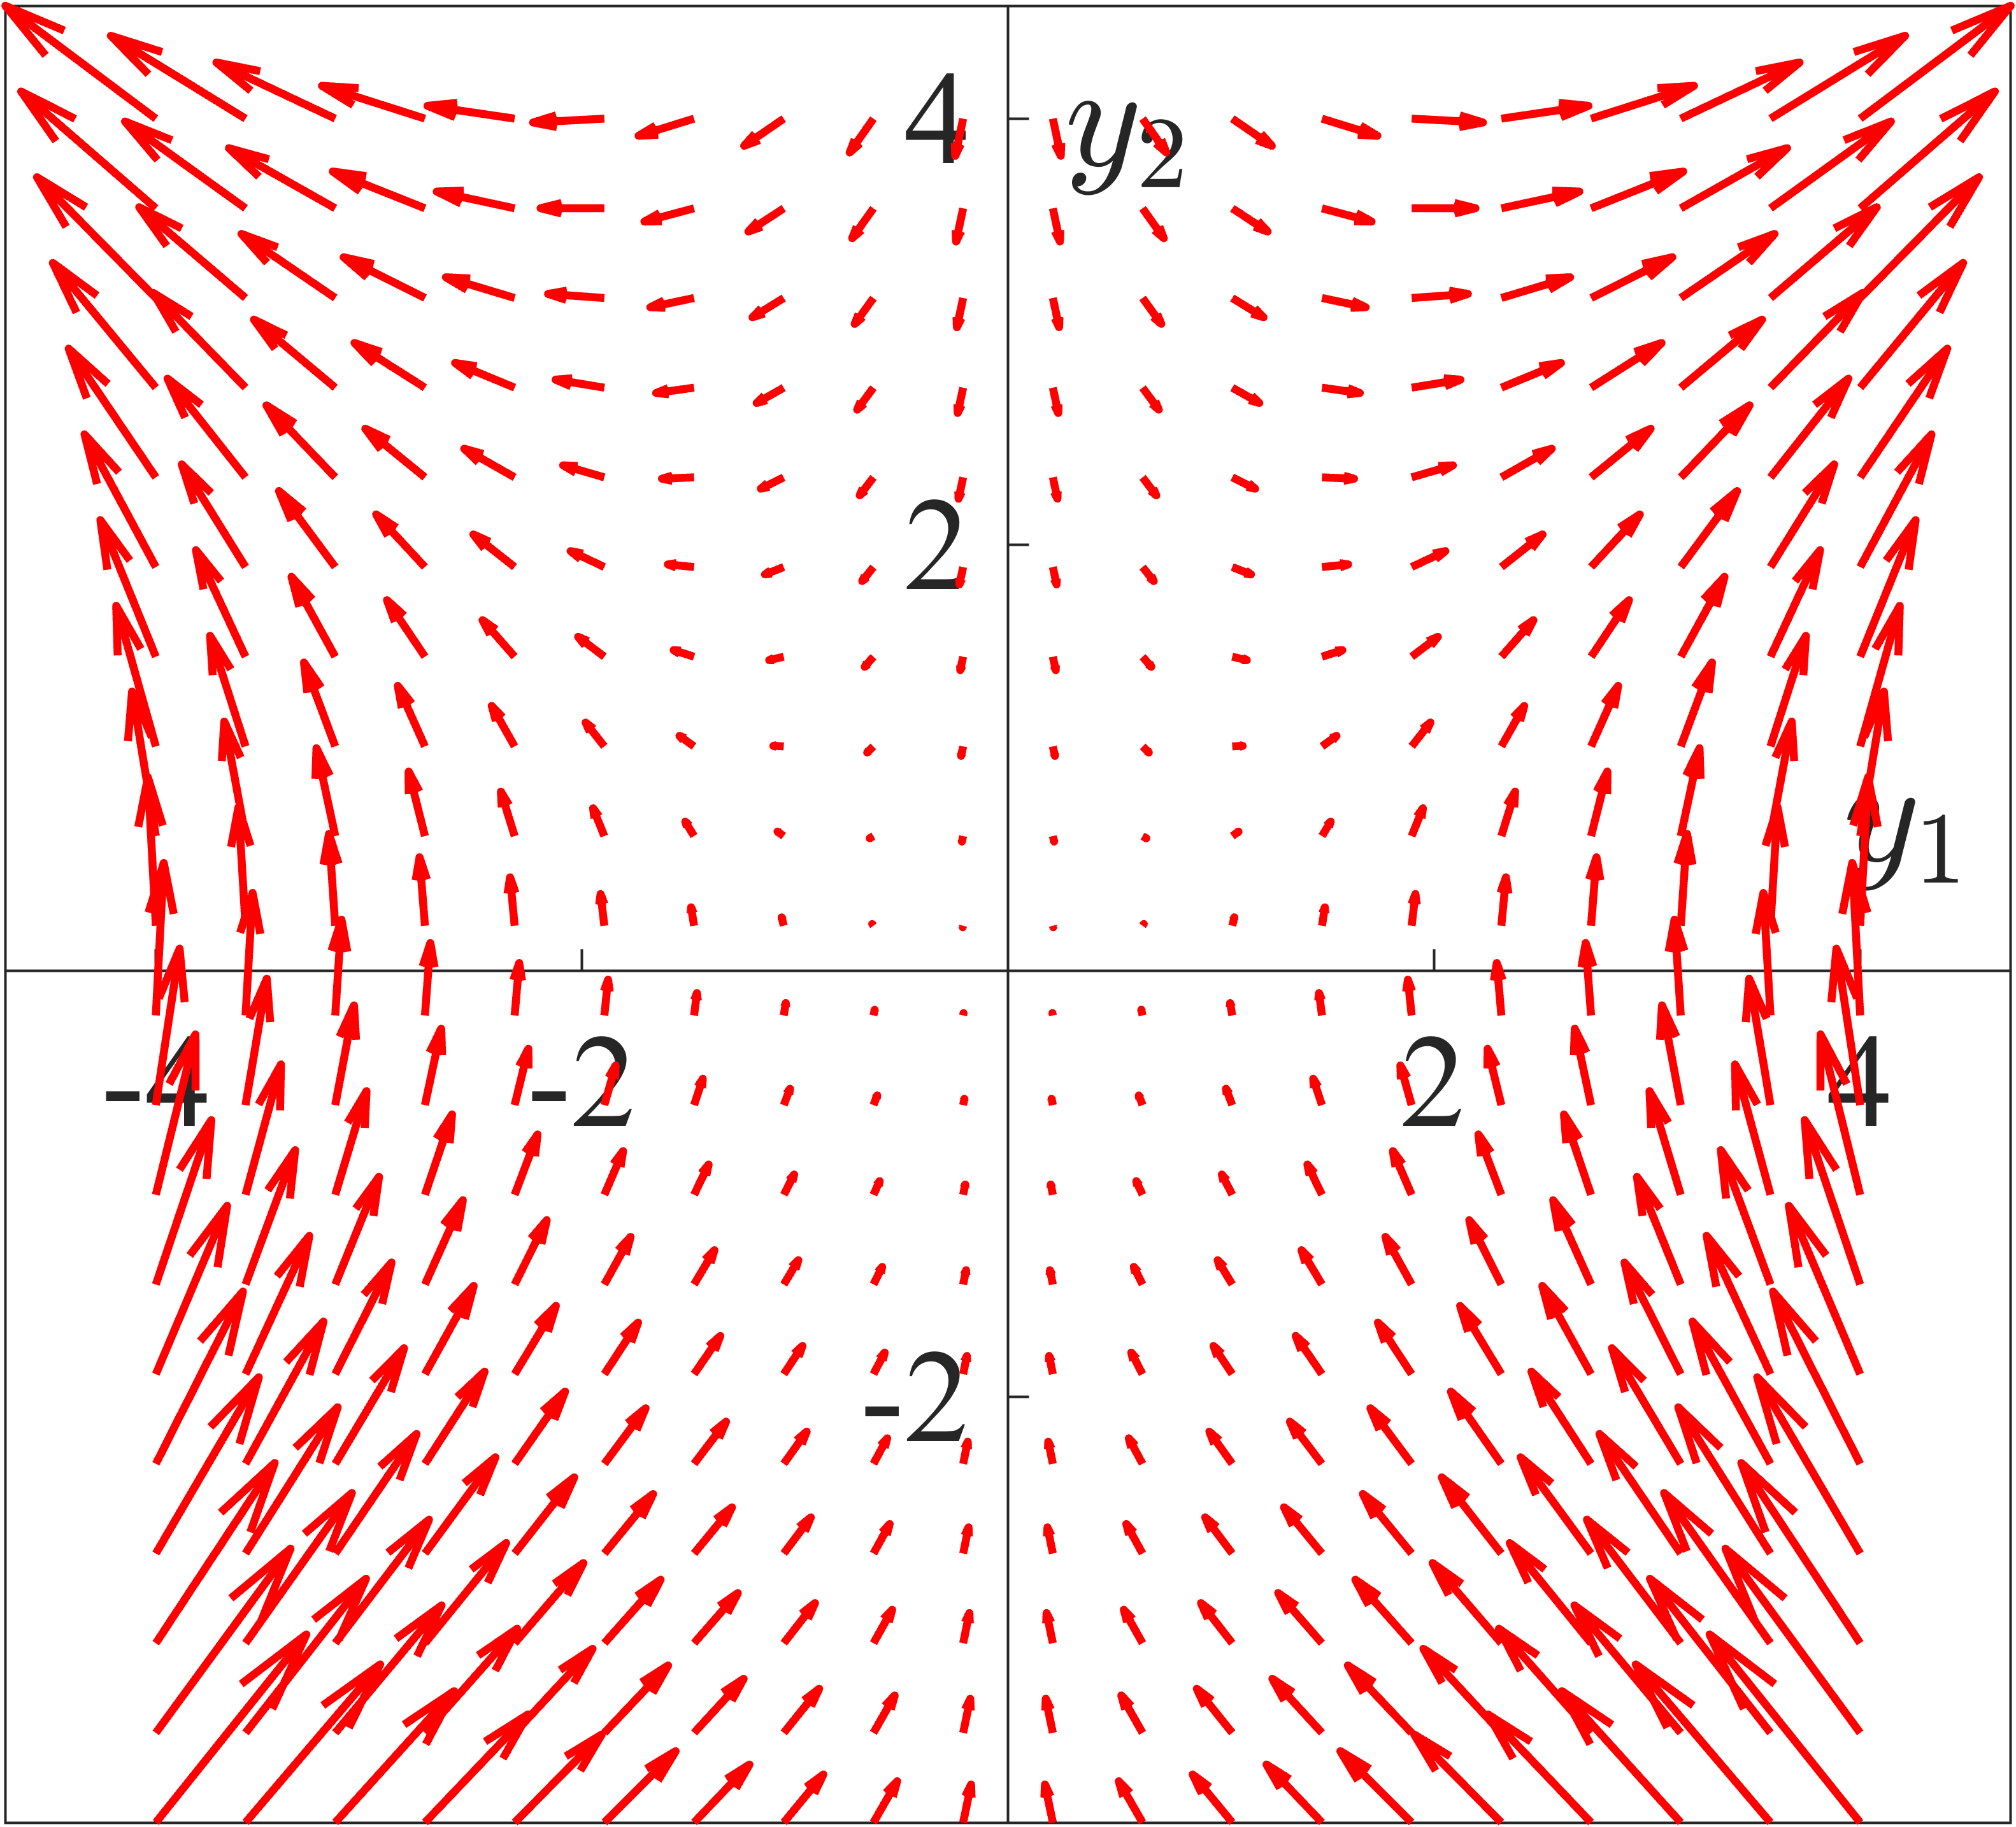
\includegraphics[width=8cm]{6.3.10.png}
\caption{Phase Portrait}
\end{figure}

\section*{Conservative Systems and Energy Functions - Pendulum 2,3}
My 3D surface plot showing the total energy function over the phase plane and my contour plot with the equilibria marked are shown below. Here I have bounded the velocity $\dot{\theta}$ by the maximum velocity for a pendulum of $v_{max} = \sqrt{2gh_{max}}$ We clearly see from the energy function and the level contours that the equilibrium is a center.
\begin{figure}[h]
\centering
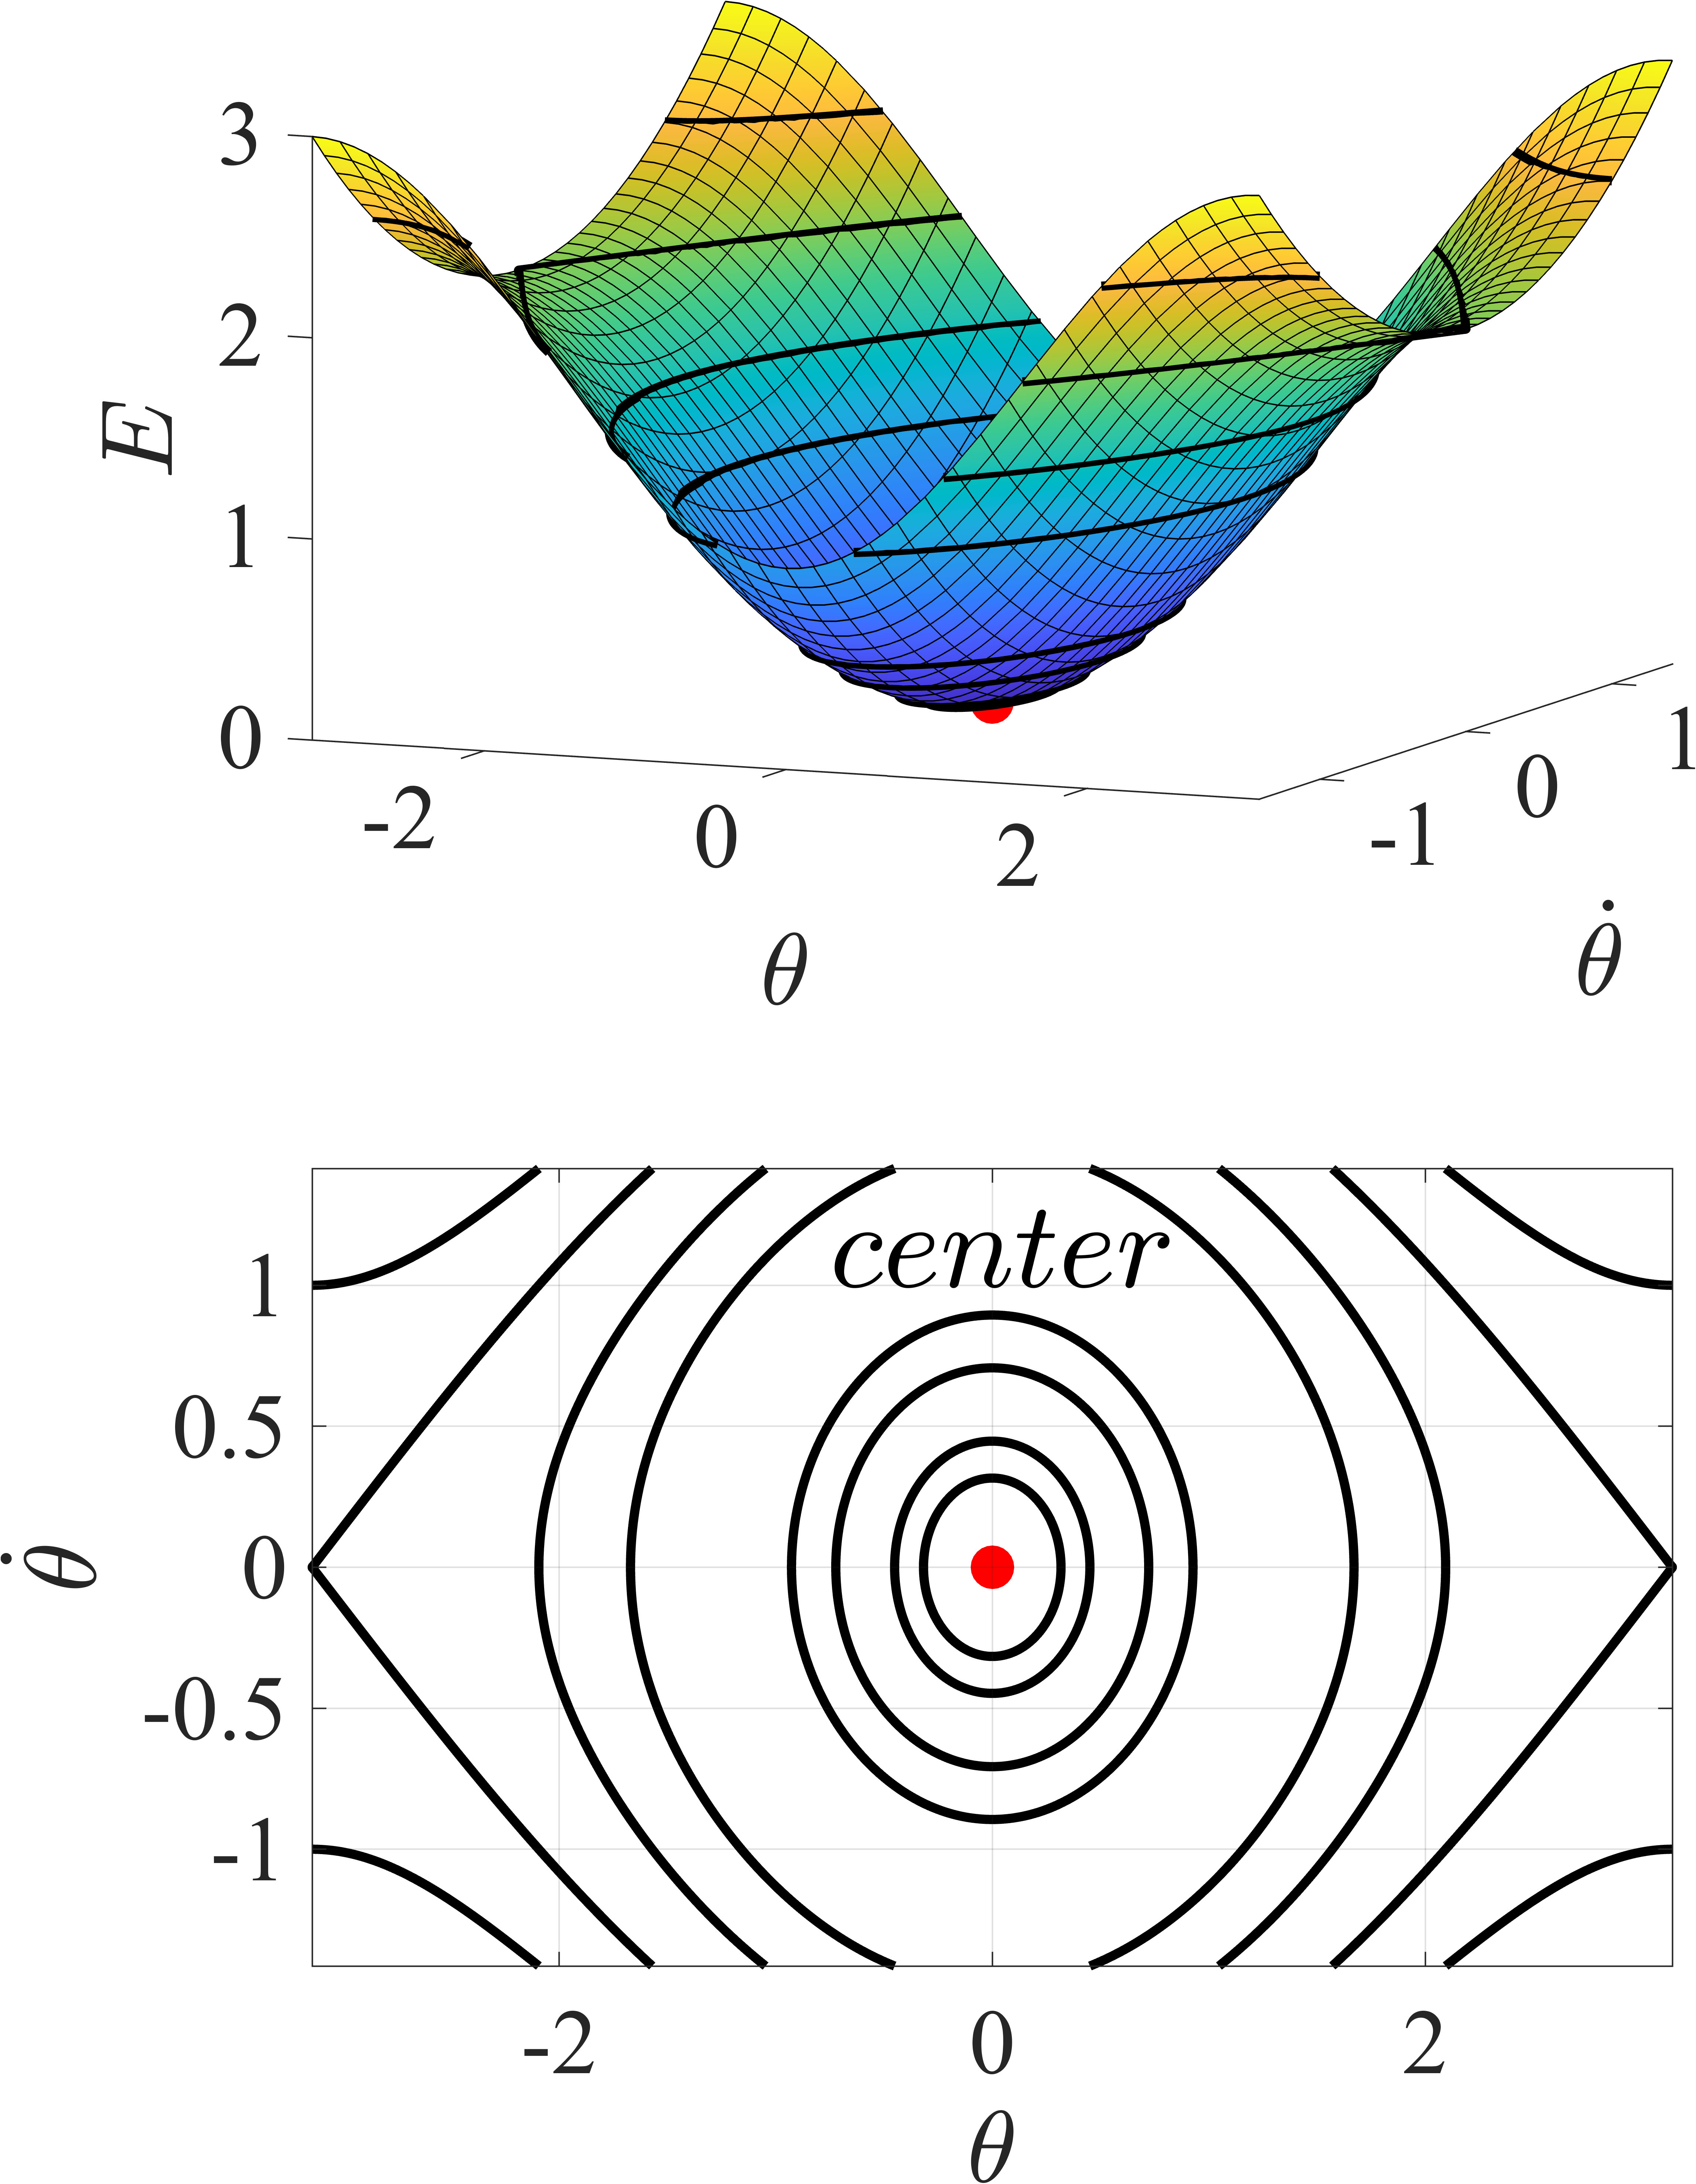
\includegraphics[width=10cm]{Conservative.2.png}
\caption{3D Surface and Level Contour Plots}
\end{figure}

\clearpage 

\section*{Two-Body Problem 7}
I plotted the energy surface and energy level contours for the given masses and angular momentum. In my plots, I marked the equilibrium with a red dot and added arrows on the level sets to indicate the direction of motion of the system. I also did this with different values of $L$ and $m$ and $M$. The original plot is shown in Figure \ref{two}. In Figure \ref{twobigL}, I increased $L$ to $L = 0.2$. We see that as the angular momentum of the system increases, the equilibrium orbital radius must also increase. In Figure \ref{twoEqM}, I made the masses equal by increasing the smaller mass $m$ to be equal to the larger mass. In Figure \ref{twoUneqM}, I made $M >> m$, in which we can approximate the system as uniform circular motion of the smaller mass $m$ around the larger mass $M$, which is approximately fixed.

\begin{figure}[h]
\centering
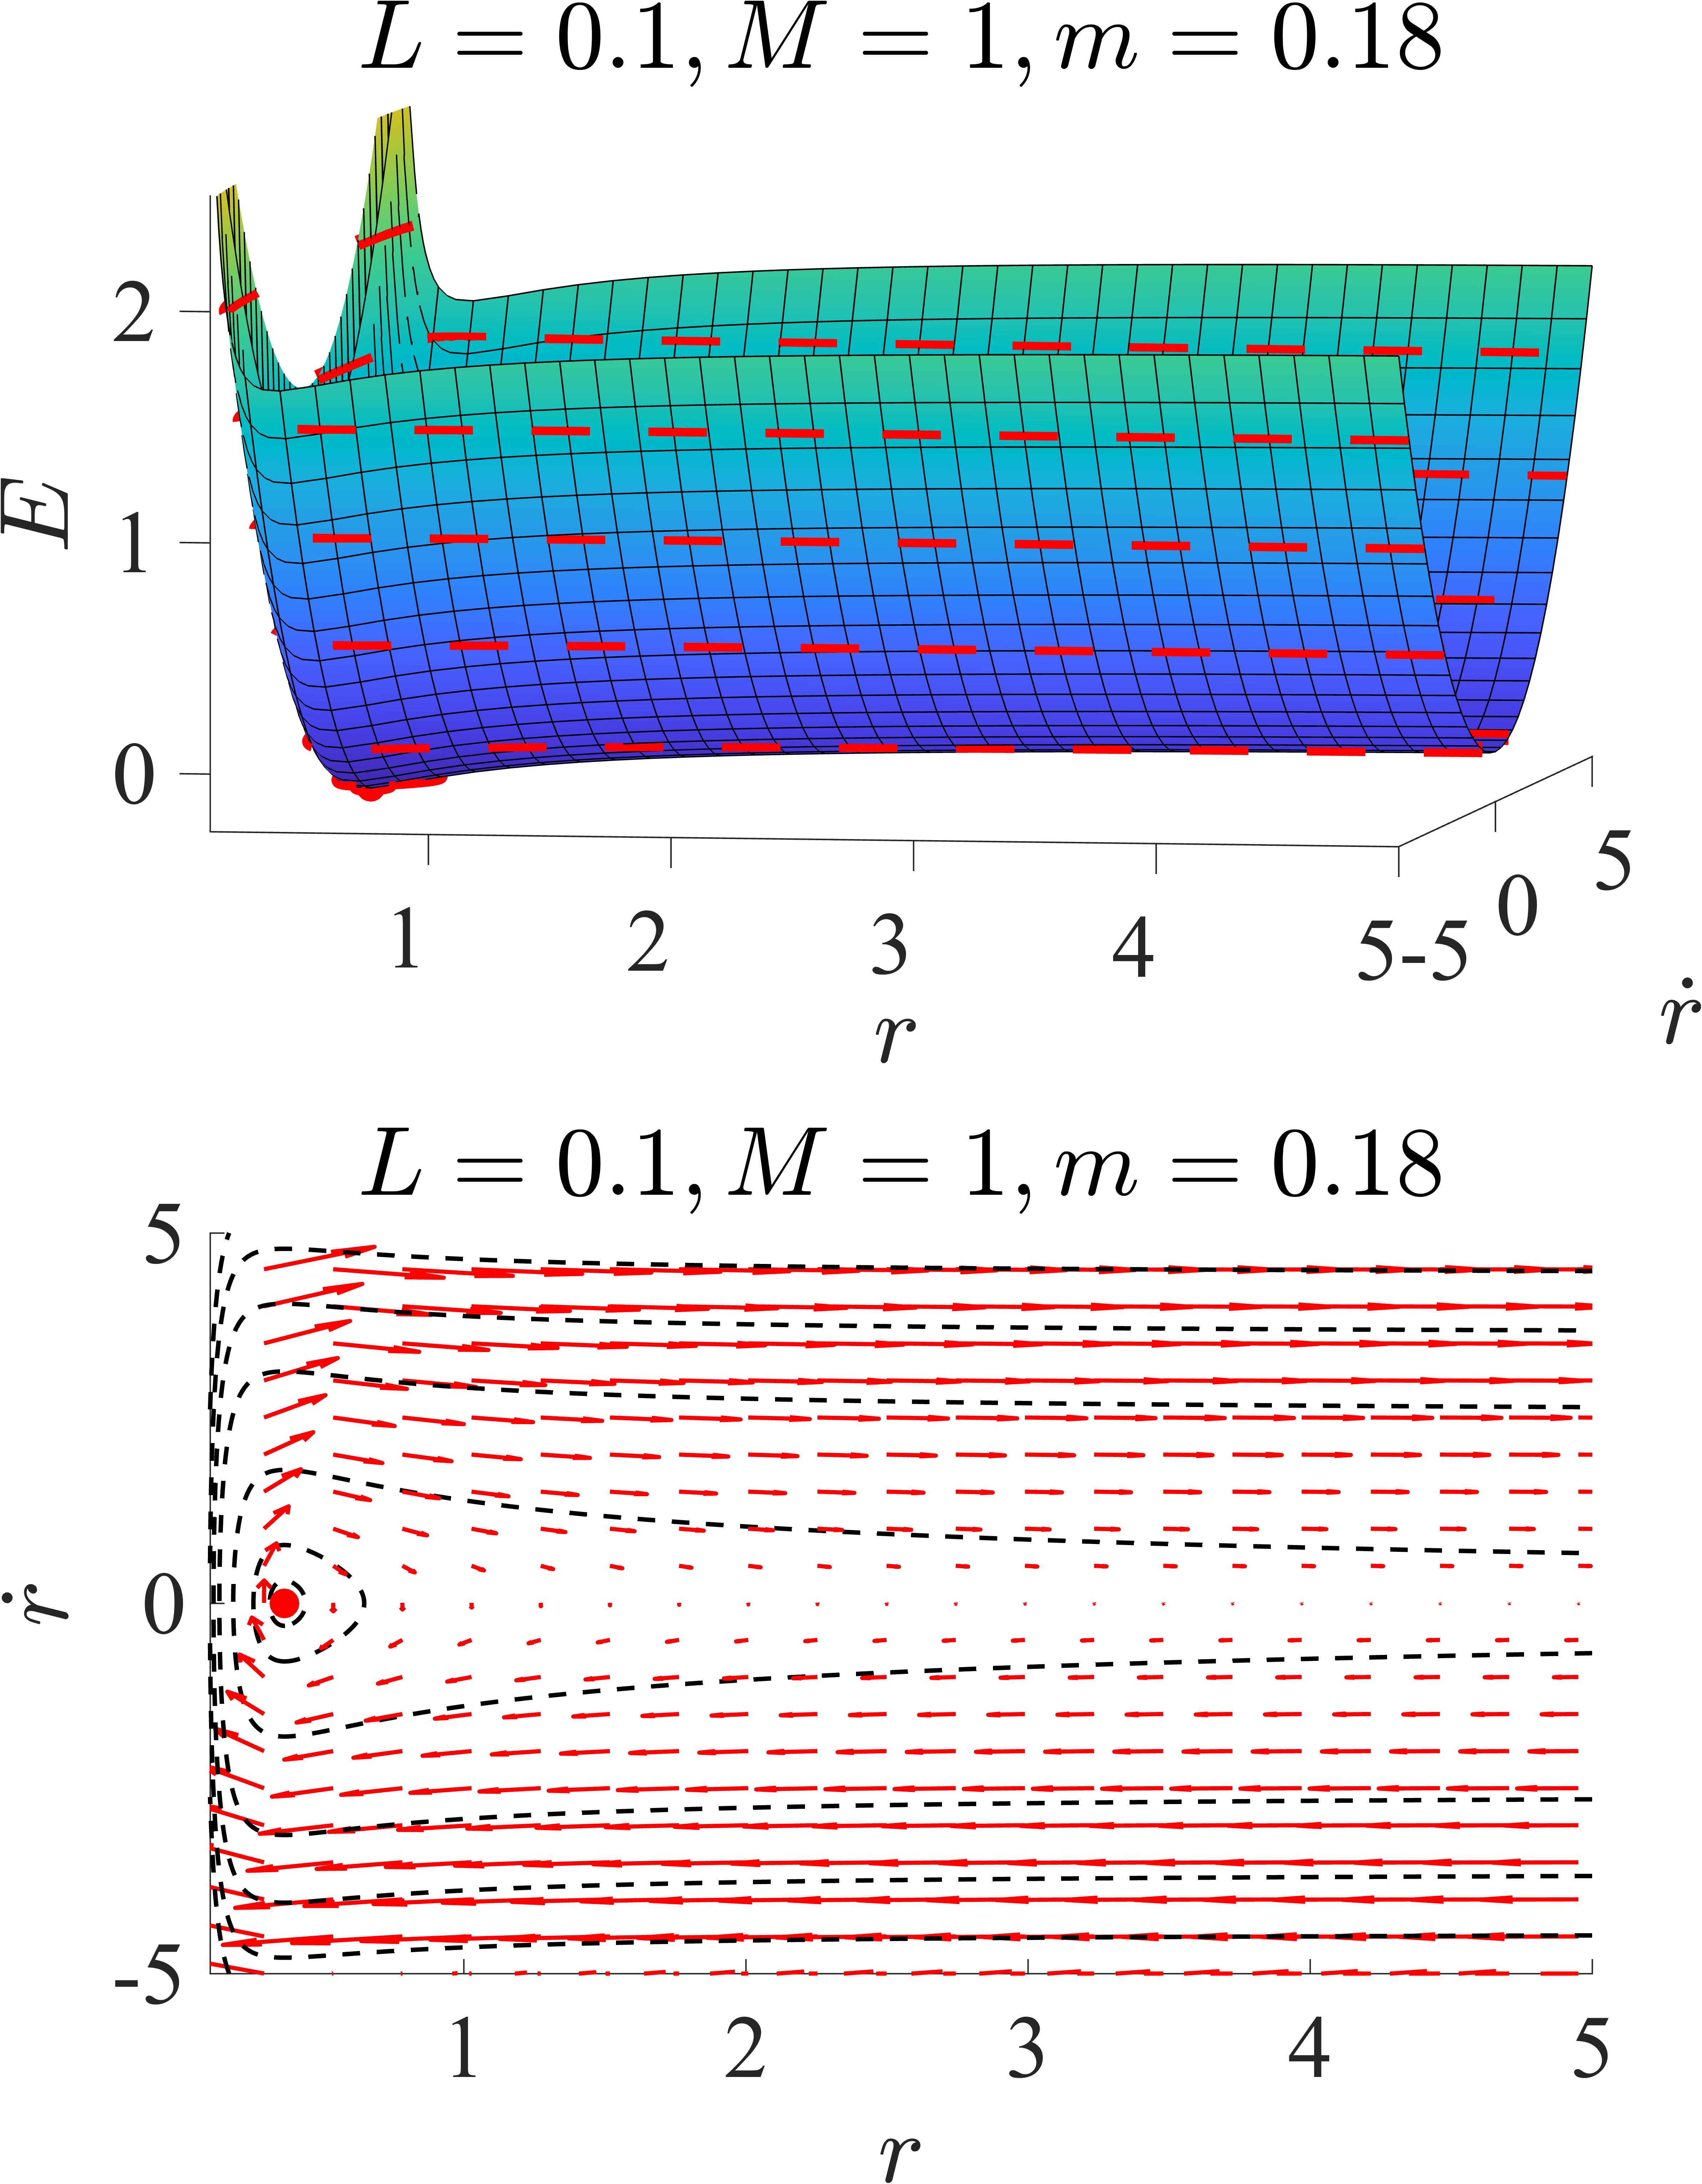
\includegraphics[width=10cm]{2 Body Problem.png}
\caption{Two-Body Problem}
\label{two}
\end{figure}

\begin{figure}[h]
\centering
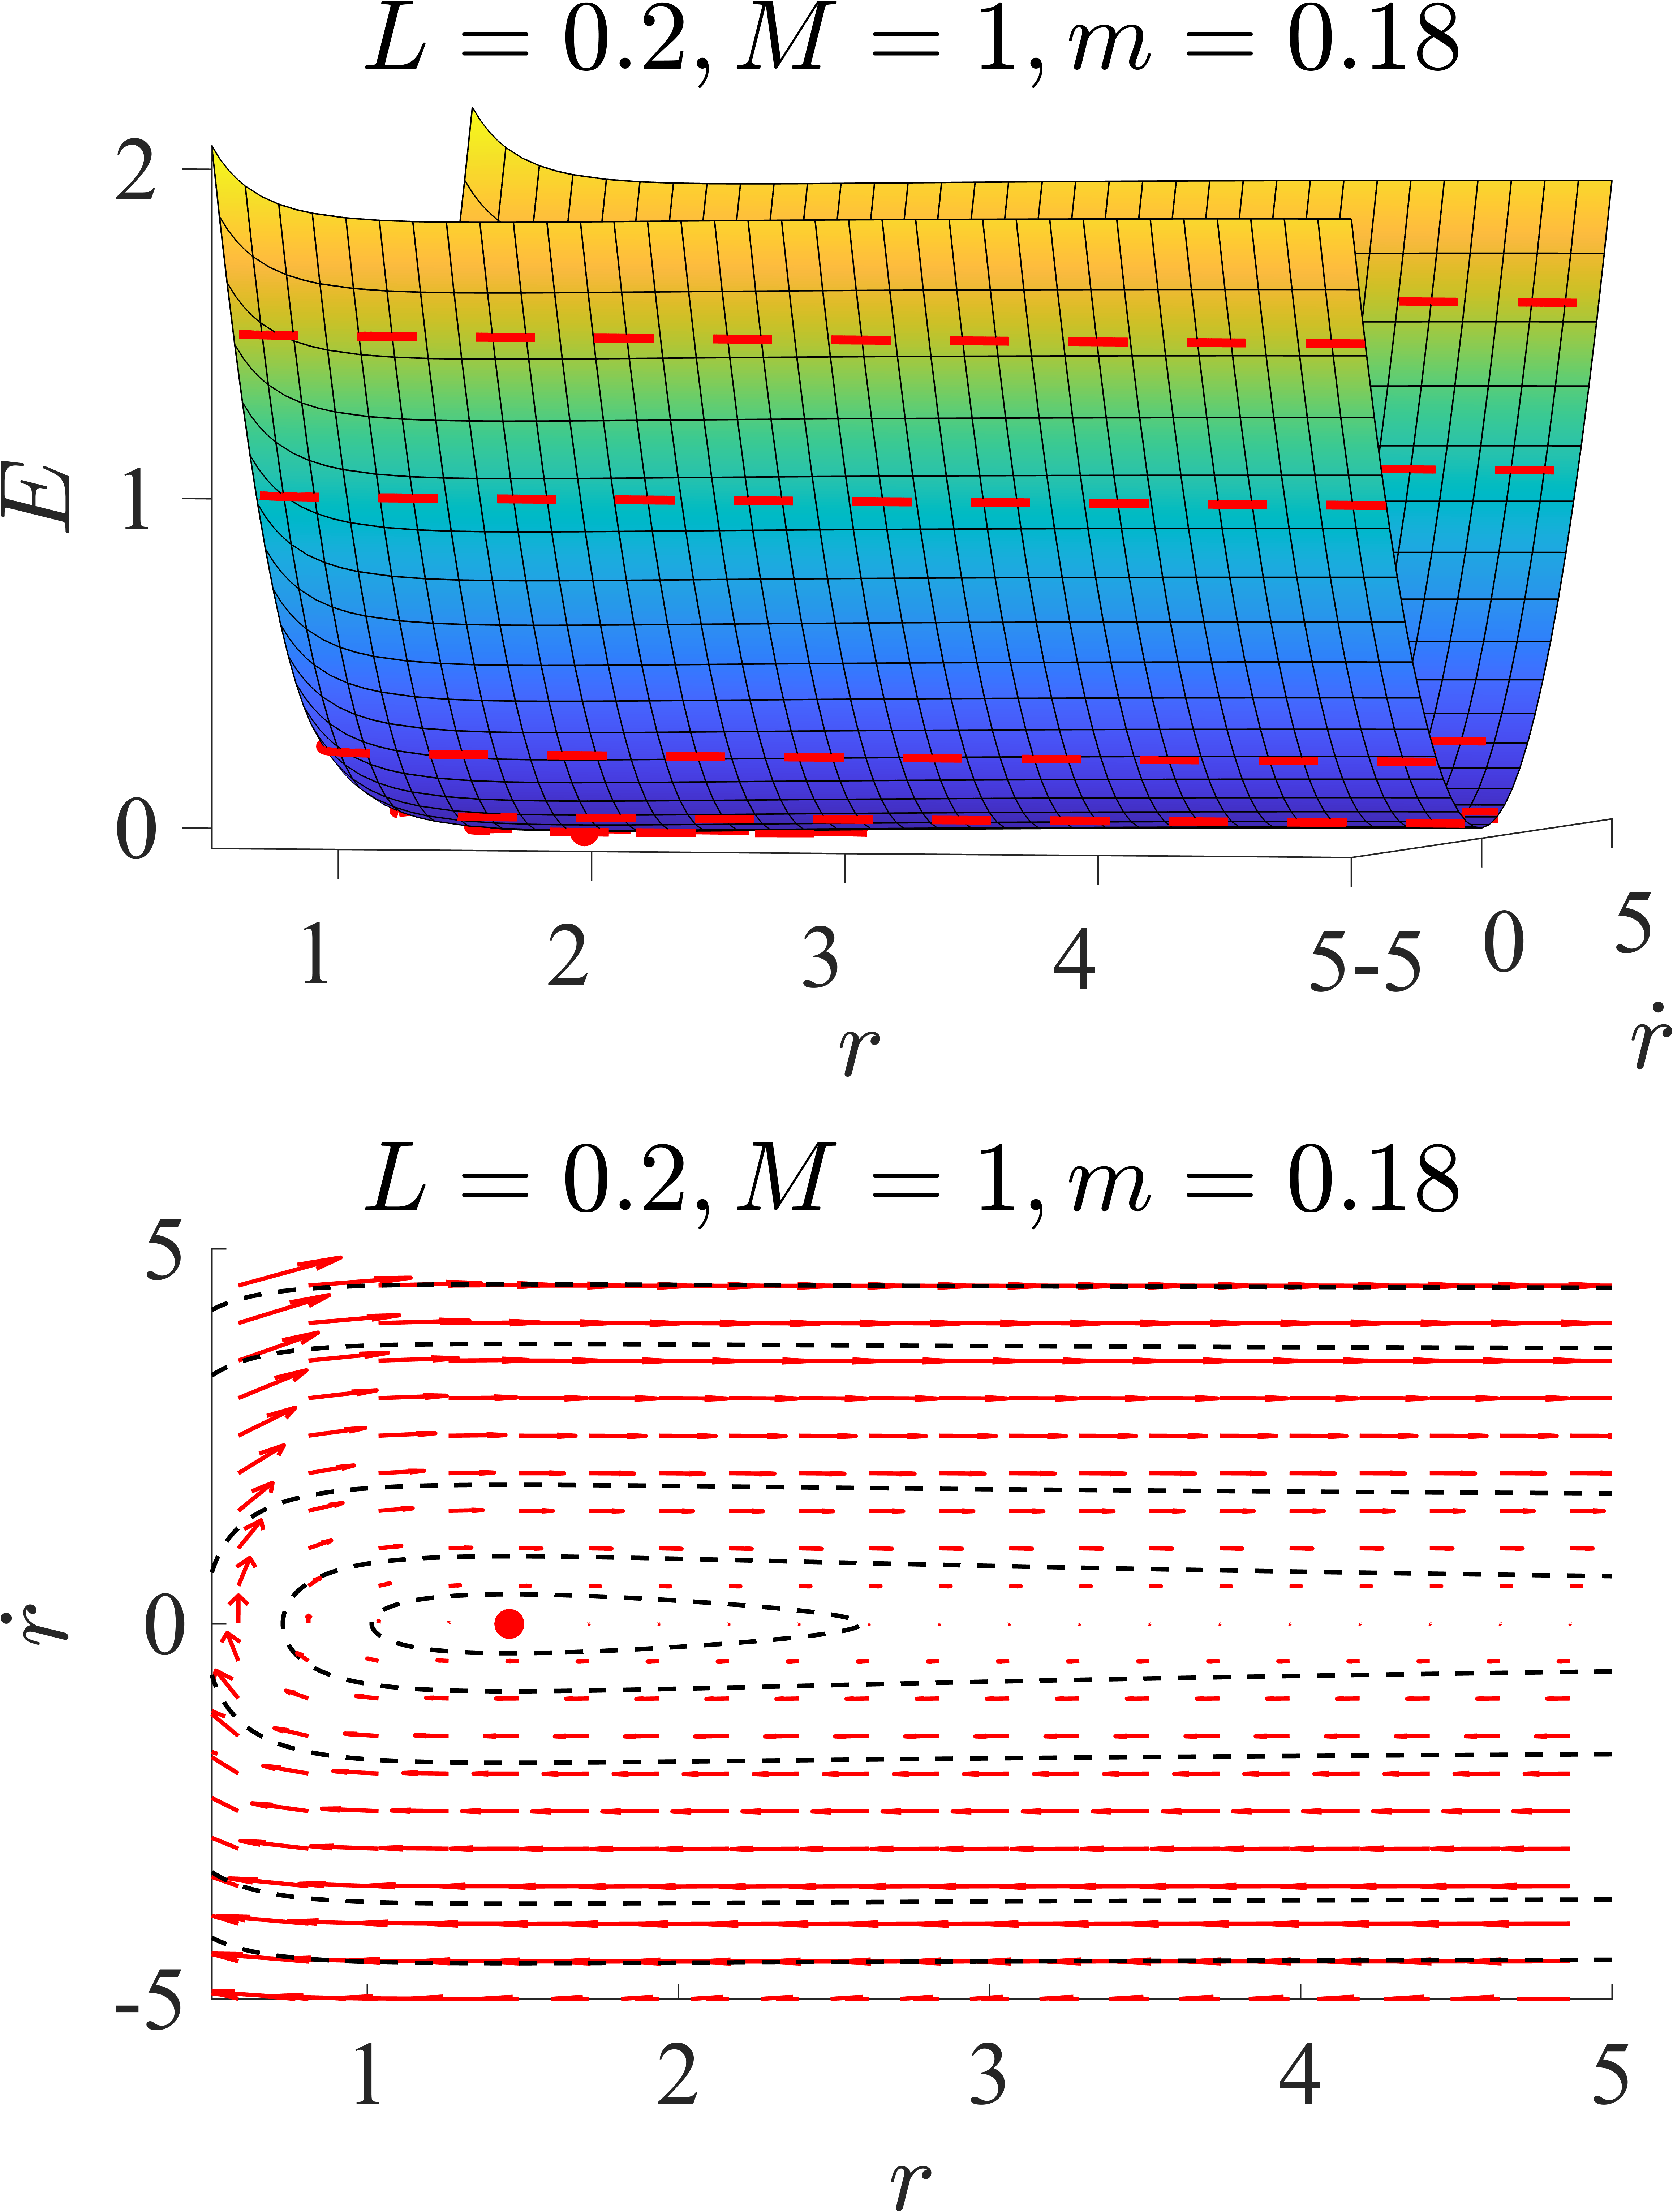
\includegraphics[width=10cm]{2 Body Problem Big L.png}
\caption{Two-Body Problem $L = 0.2$}
\label{twobigL}
\end{figure}

\begin{figure}[h]
\centering
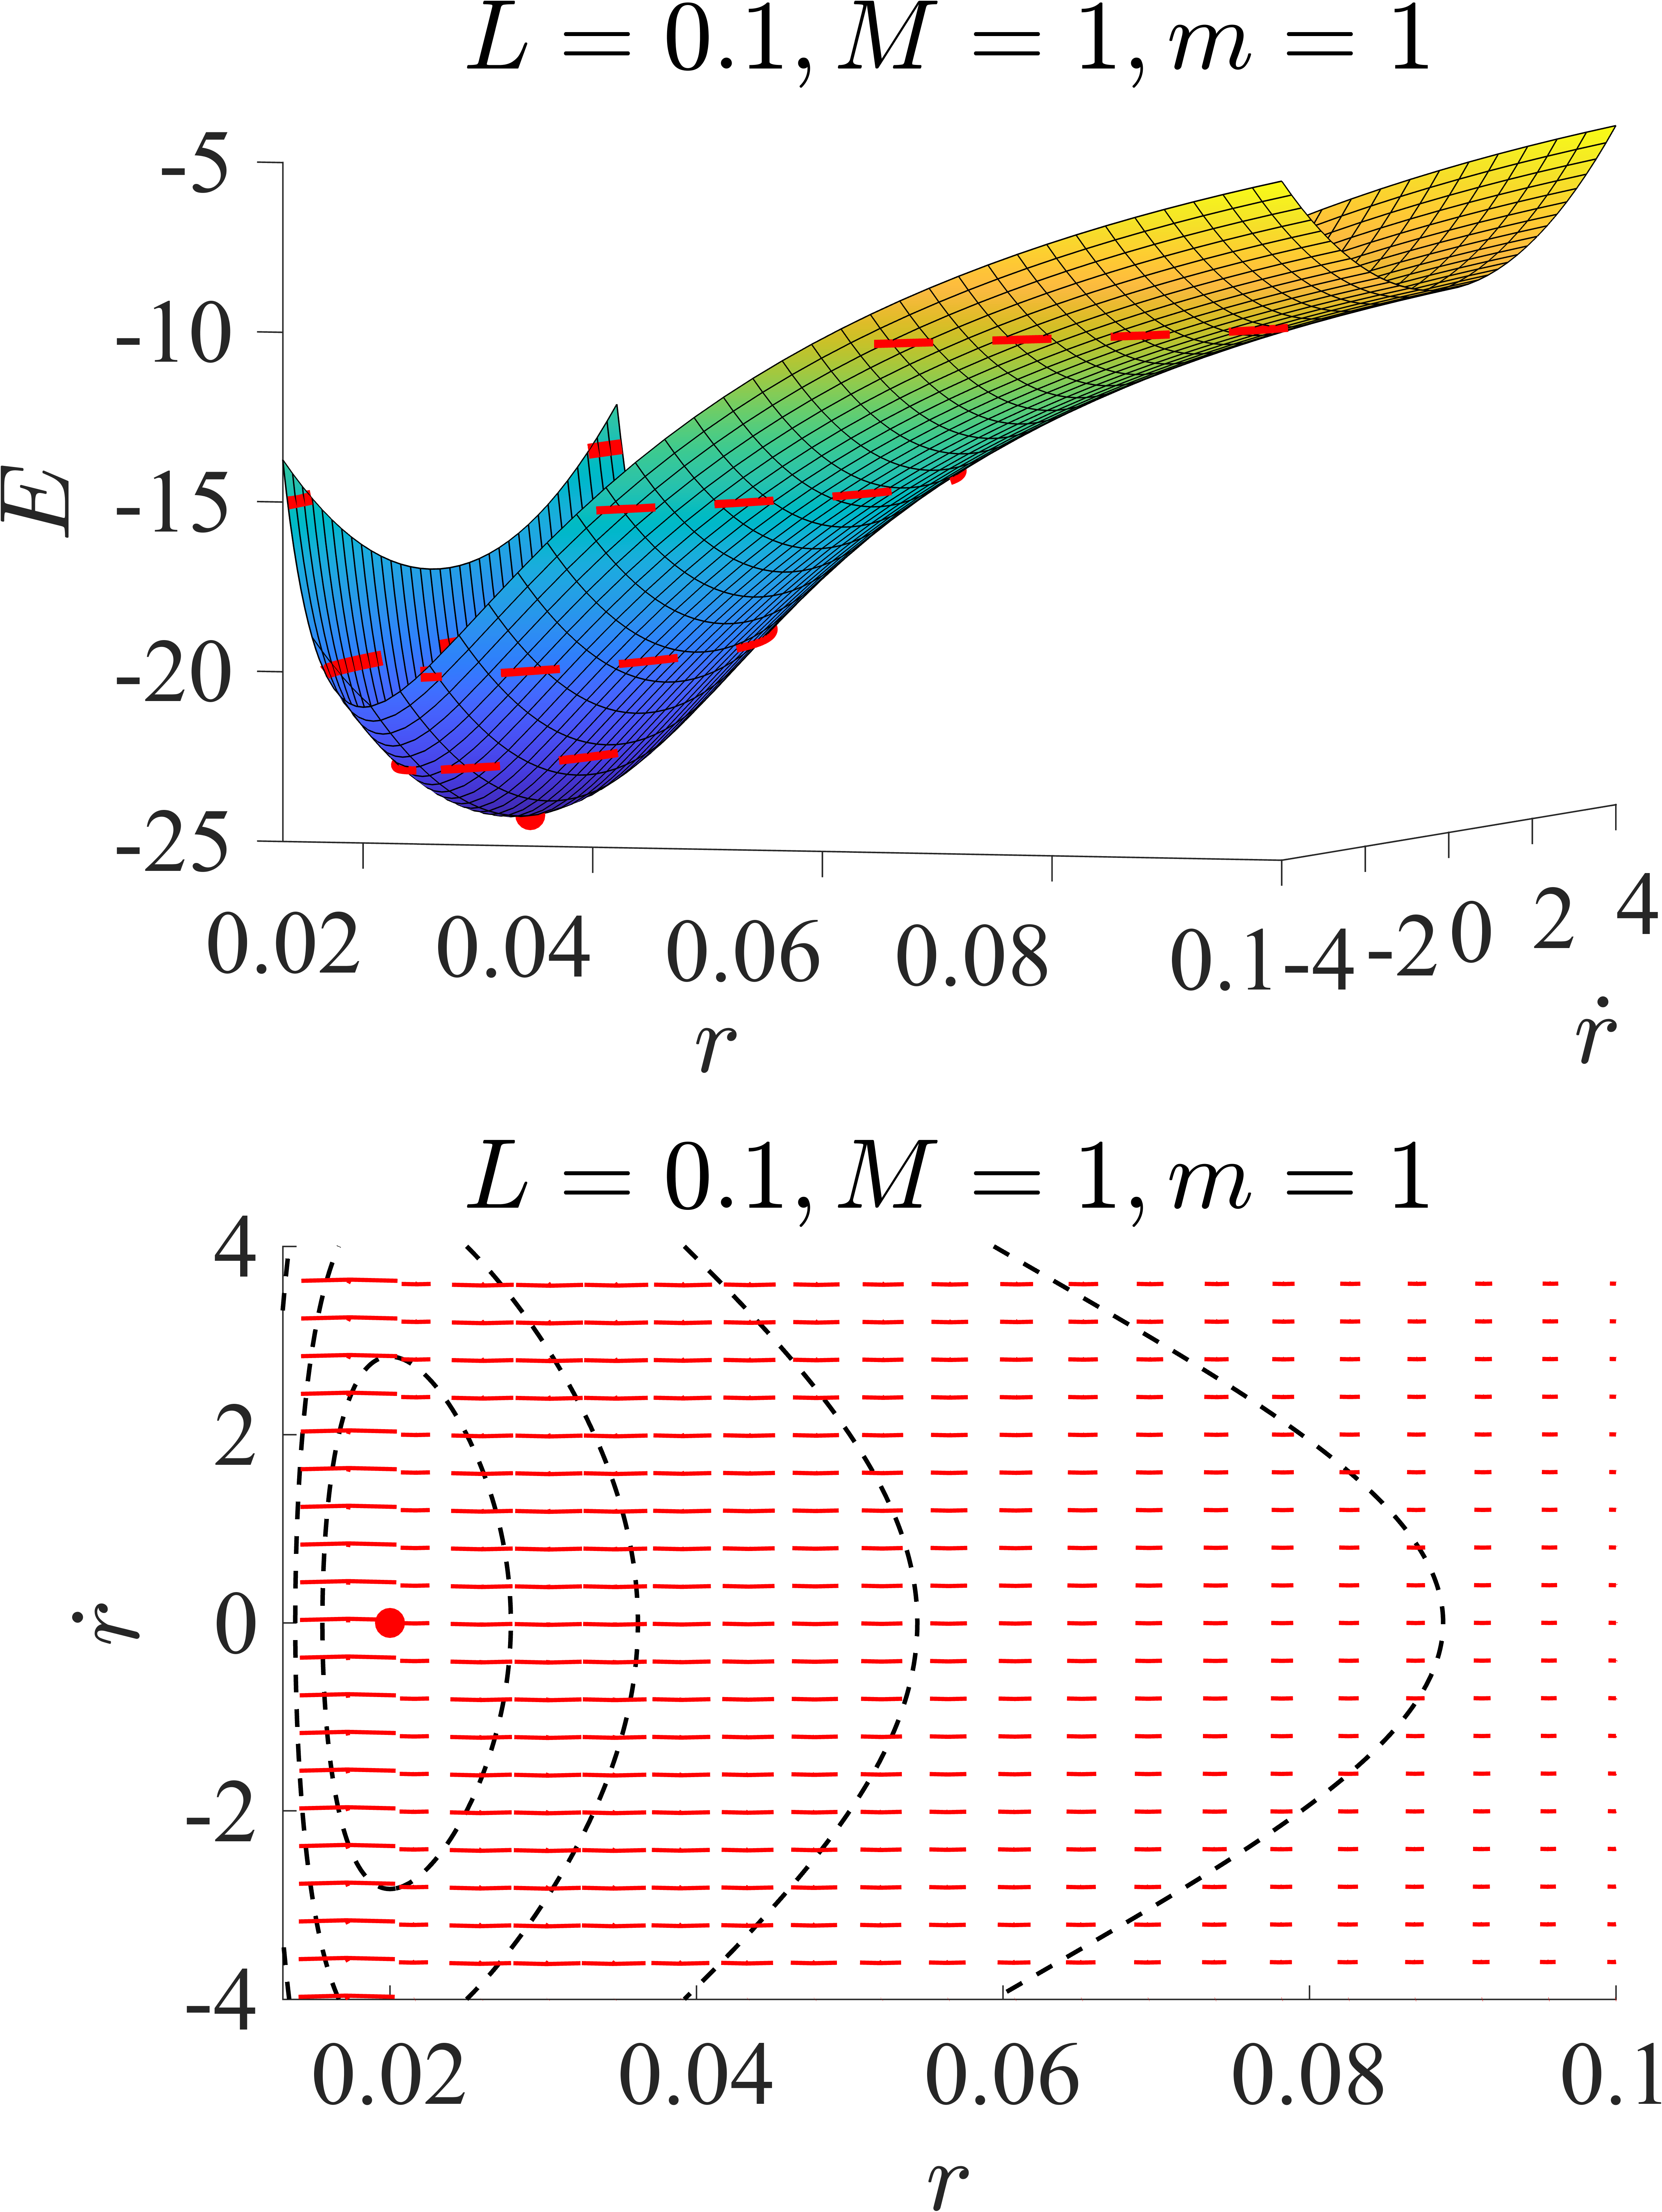
\includegraphics[width=10cm]{2 Body Problem Equal Masses.png}
\caption{Two-Body Problem Equal Masses}
\label{twoEqM}
\end{figure}

\begin{figure}[h]
\centering
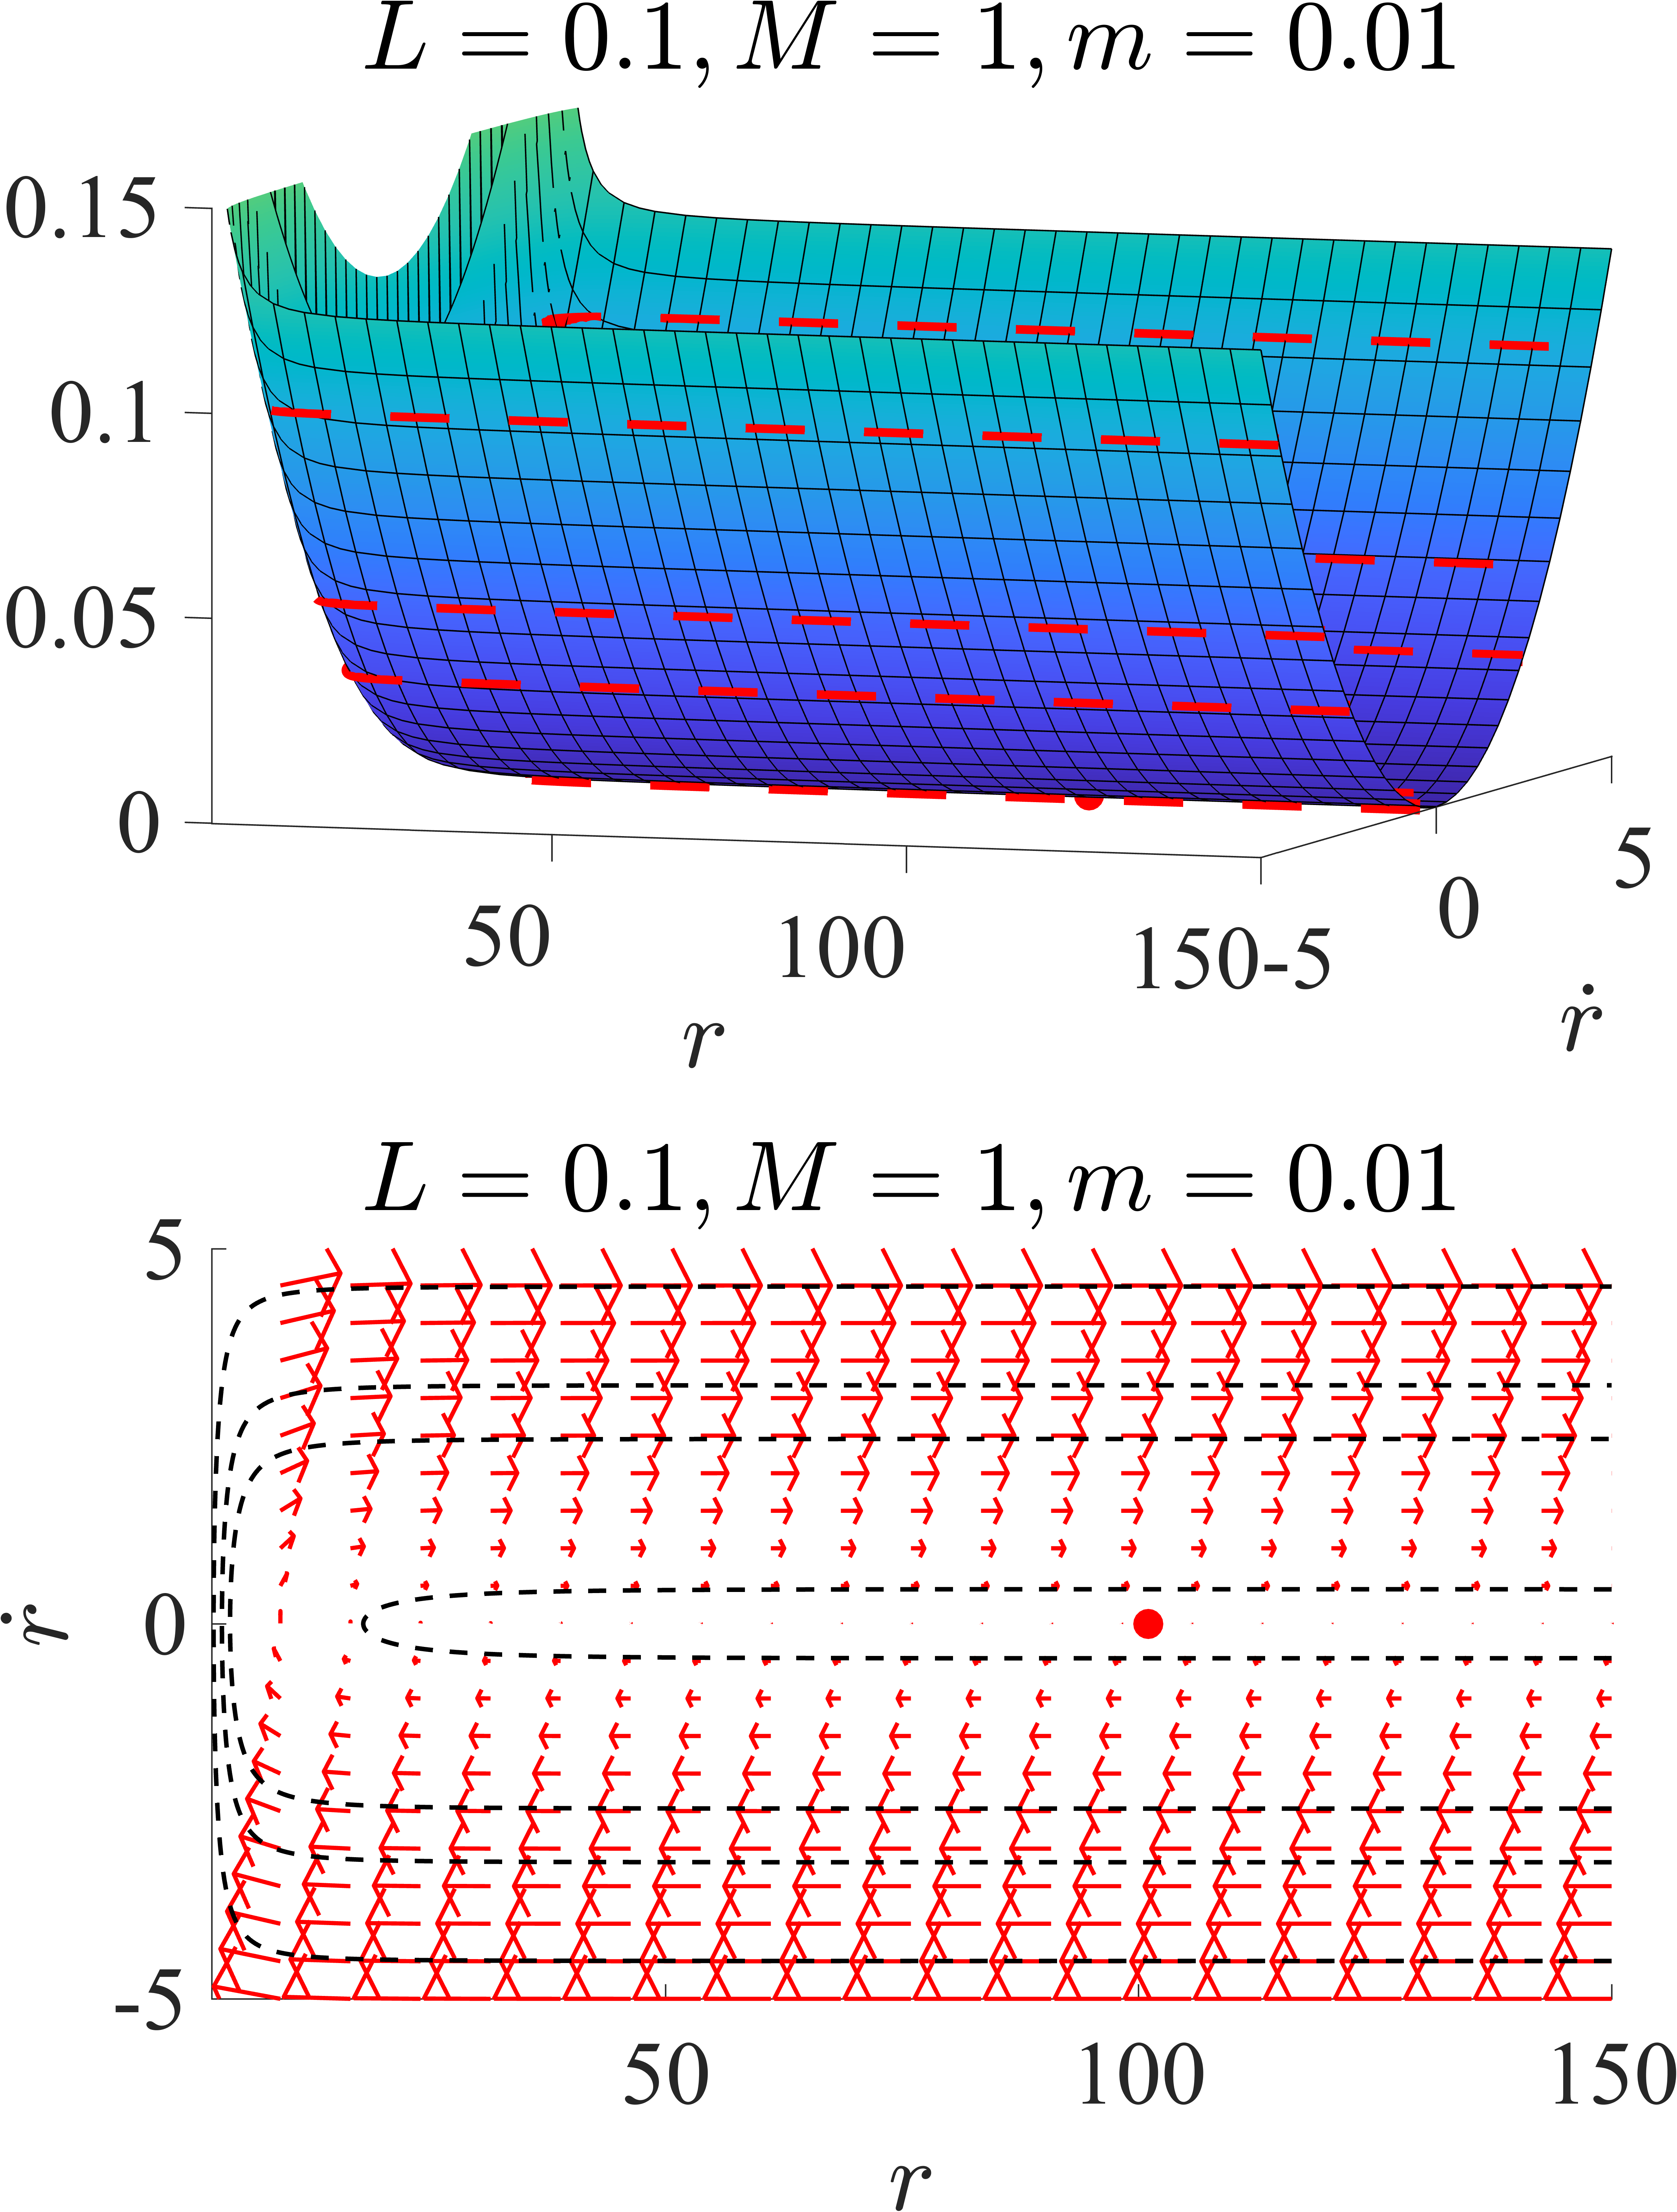
\includegraphics[width=10cm]{2 Body Problem Unequal Masses.png}
\caption{Two-Body Problem $M >> m$}
\label{twoUneqM}
\end{figure}

\clearpage

\section*{Two-Body Problem 8}
I plotted the energy contour in Figure \ref{zero}, in which the level set for $E = 0$ is the black contour. I also plot a trajectory at negative energy in cyan, and I plot a trajectory at positive energy in magenta. Since kinetic energy must always be positive (if the planets are moving at all), then a negative energy must mean that the potential energy is greater than the kinetic energy. We see that at negative energy, the level sets form elliptical shapes in which the planets get farther and closer together in an elliptical orbit. At the positive energy level set, the planets seem to be just getting closer or farther away from each other, in which $\dot r$ stays constant but $r$ increases to infinity as time increases to infinity. In this case, the initial kinetic energy must be greater than the initial potential energy. At the zero energy level set, we see that as $r$ increases, $\dot r$ decreases, which means that the radial velocity will become smaller and smaller, so the planets will go farther apart at a slower and slower rate. This corresponds to a system in which at $r = \infty$, the planets have zero potential energy and zero kinetic energy. Then as potential energy becomes more negative as the planets get closer, kinetic energy also increases, and as potential energy increases (less negative as the planets get infinitely far away), kinetic energy decreases to 0.

\begin{figure}[h]
\centering
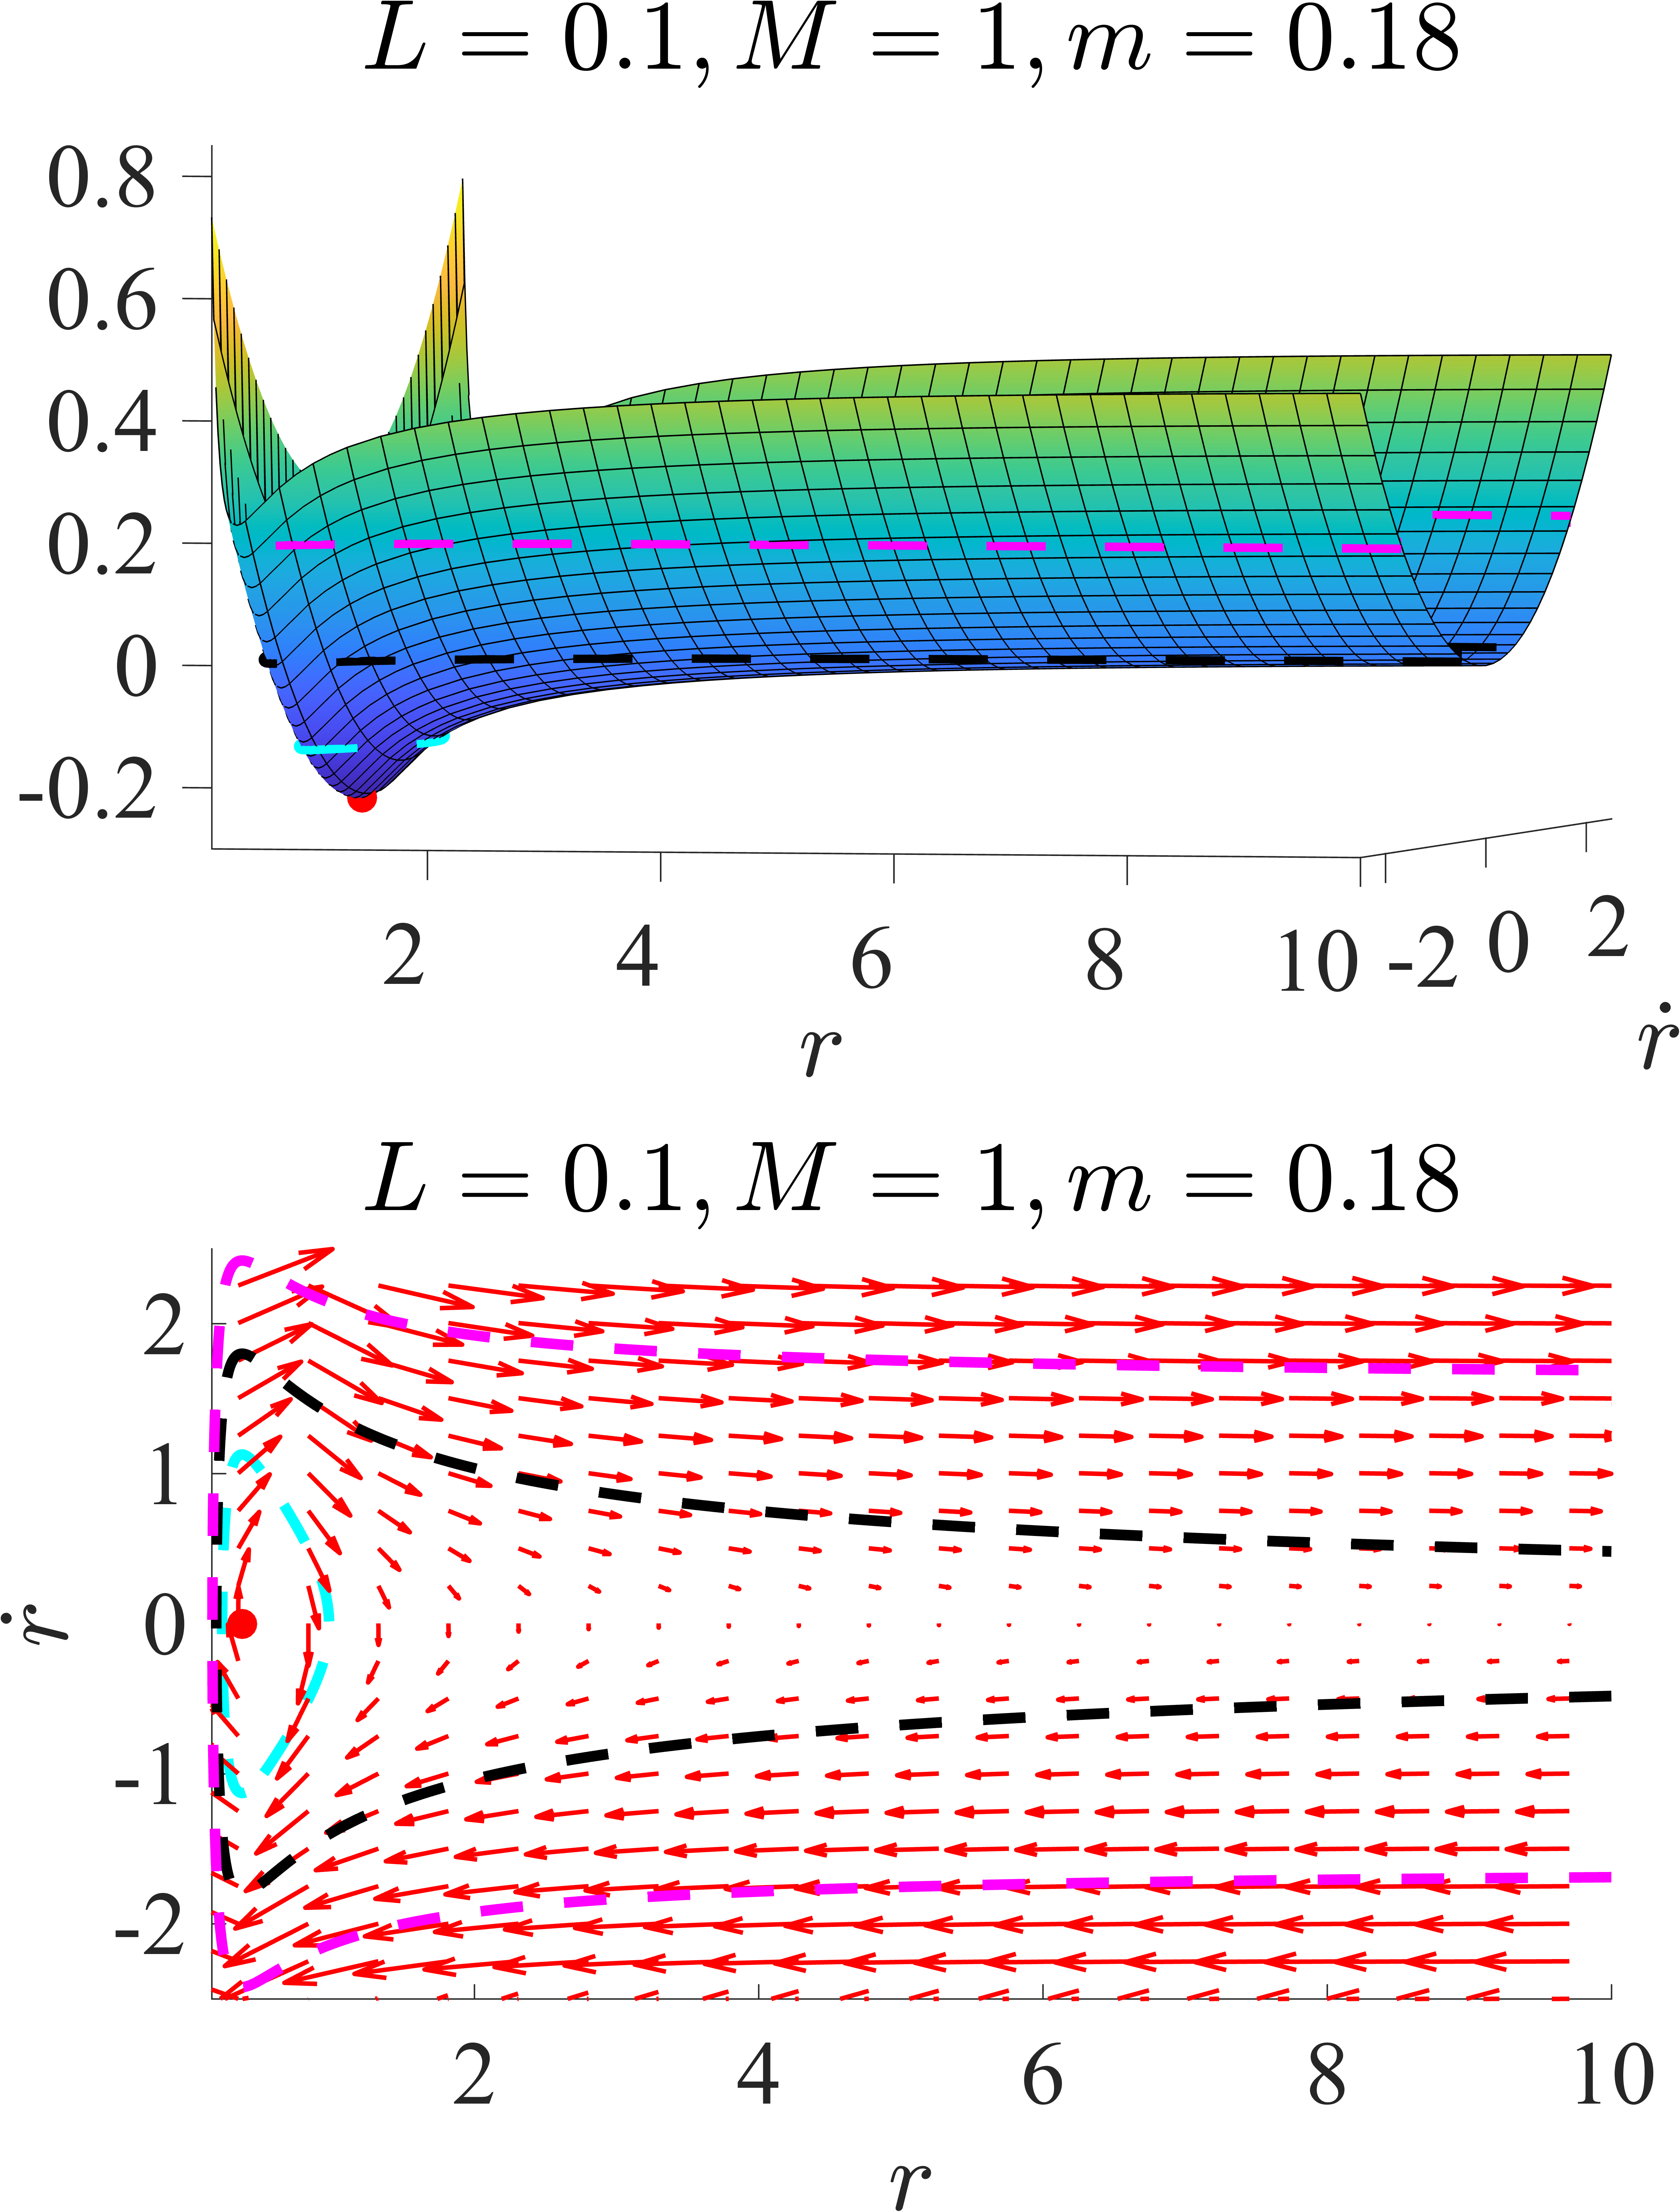
\includegraphics[width=10cm]{2 Body Problem Zero Energy.png}
\caption{Two-Body Problem With Zero Energy Contour}
\label{zero}
\end{figure}

\clearpage

\section*{Three-Body Problem 5}
I plotted the potential function using simplified parameters of $M_S = 100$, $M_E = 5$, $r_E = 10$, $G = 1$, $\omega = \sqrt{G(\frac{M_S + M_E}{r_E^3})}$. My plot is shown below:

\begin{figure}[h]
\centering
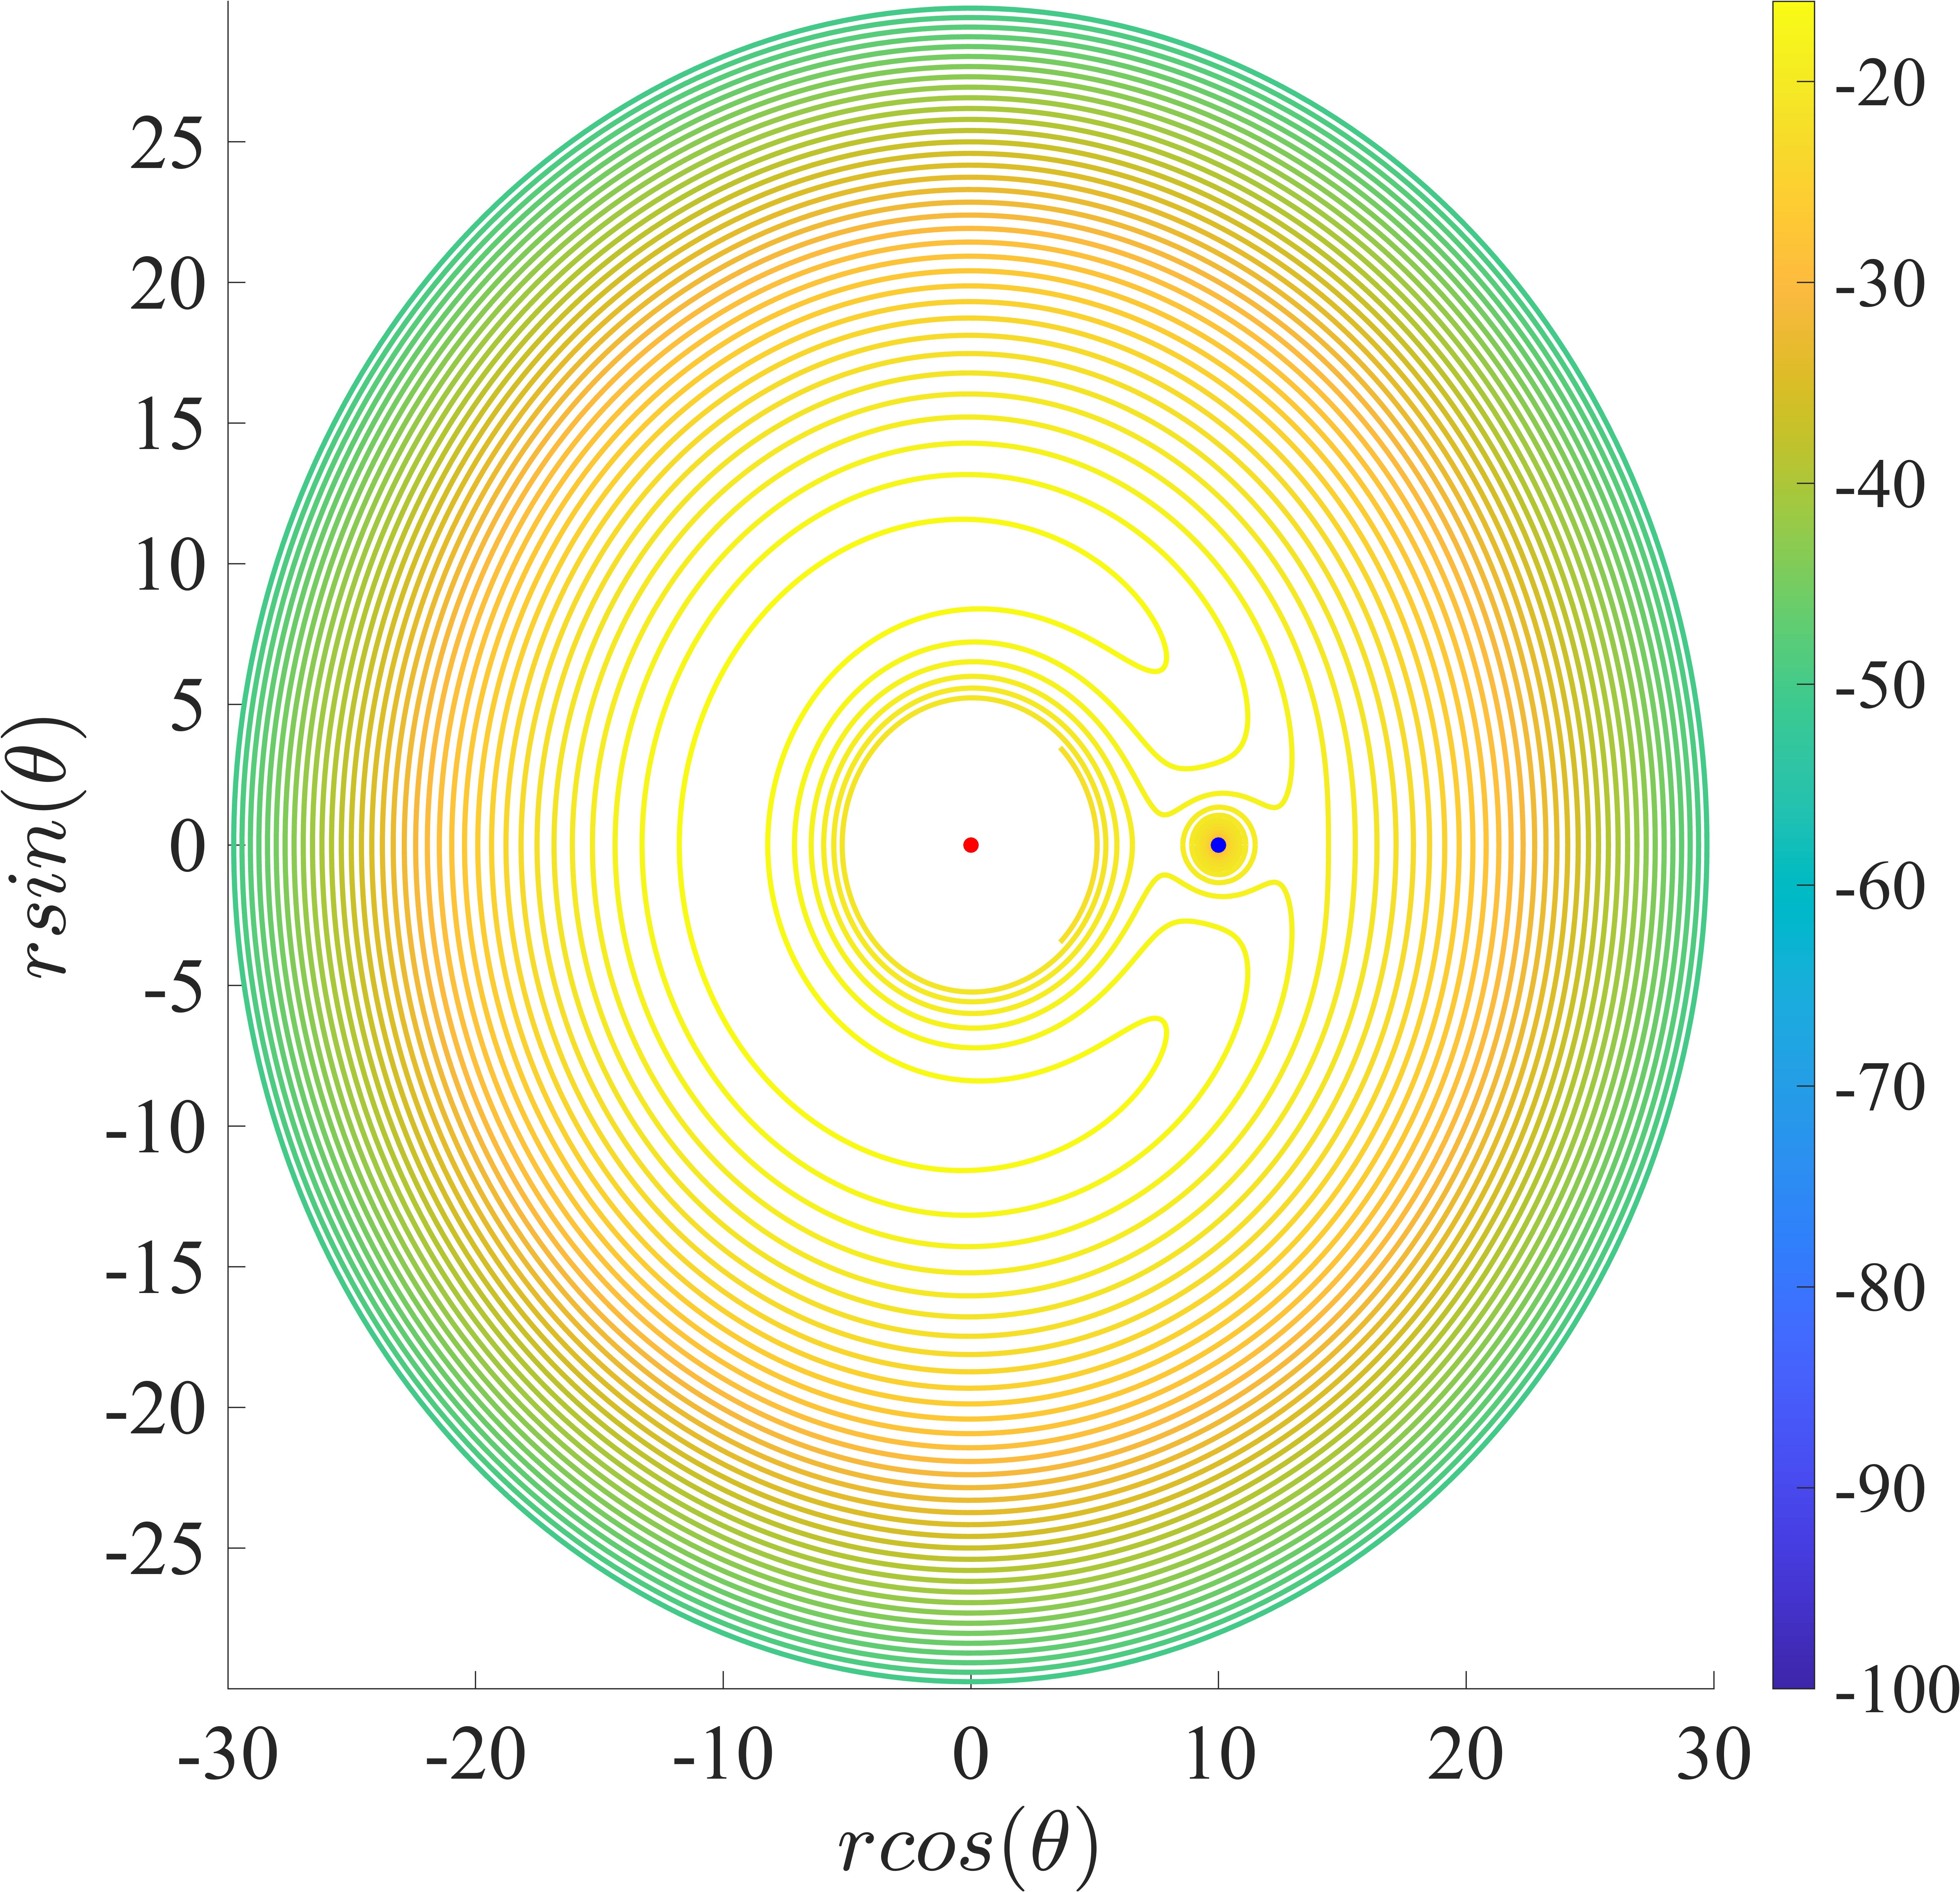
\includegraphics[width=10cm]{three_body_prob.png}
\caption{Three-Body Problem with Simplified Parameters}
\label{zero}
\end{figure}

There are supposed to be 5 Lagrange points here. I can clearly see 3 of them, but L4/L5 aren't appearing. Using the physical constants, I am unable to get the Lagrange points to clearly appear because the very large gravitational potential of the sun is masking the effects of the gravitational potential of the centrifugal force.

\begin{figure}[h]
\centering
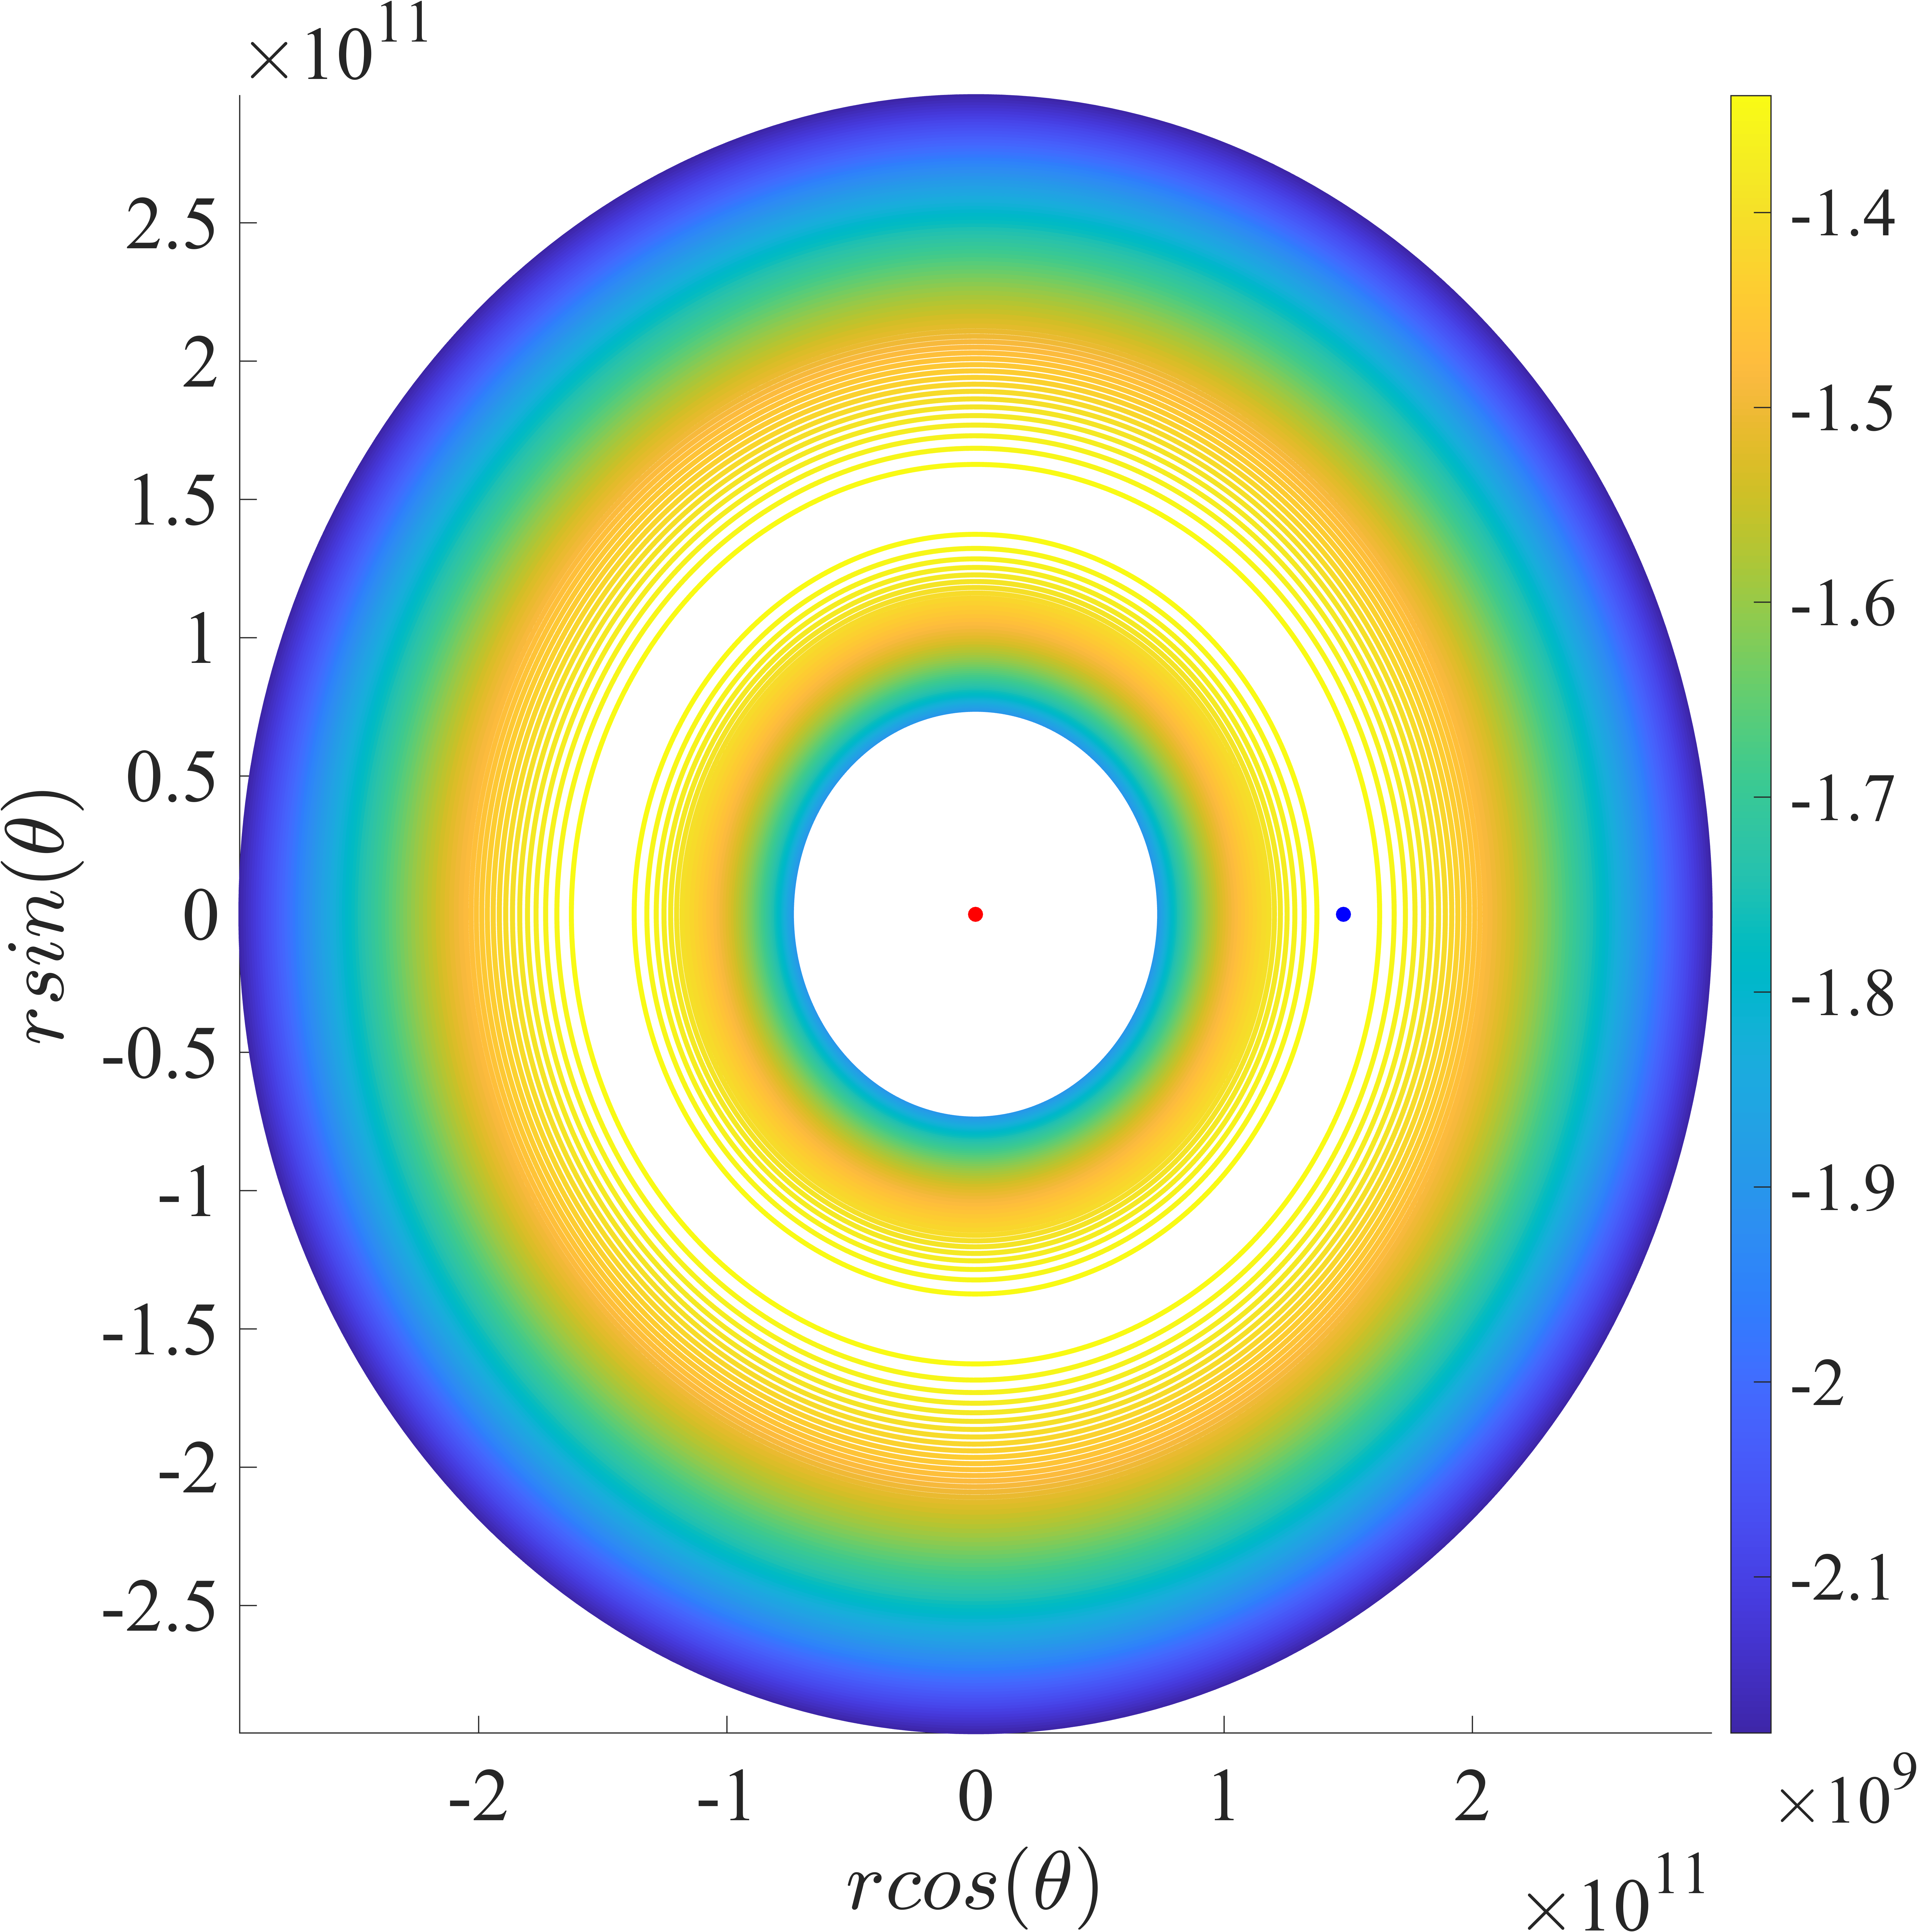
\includegraphics[width=10cm]{three_body_prob_phys.png}
\caption{Three-Body Problem with Physics Parameters}
\label{zero}
\end{figure}
 
Since we are plotting the potential, the system moves to minimize the potential energy. Contours depict regions of constant potential. The telescope will move across (perpendicular) to the contours to minimize its potential. We can see this in the governing equation for our system, in which $\frac{d^2}{dt^2} x(t) = - \nabla V(x)$, which means that the telescope will move in the direction that is opposite of the gradient of the potential function. This is the direction down the gradient along which the potential function decreases most quickly.

\section *{Three-Body Problem 6}
There are supposed to be 5 Lagrange points, of which 3 (L1/L2/L3) are unstable saddle points, 2 (L4/L5) are stable local maxima (stability is due to the Coriolis force). In the potential function, there are minima near the earth and sun, as these correspond to the gravitational potential energy terms with a very small radius from either planet. 

\clearpage
\section{Code}
This is all of my code for this homework.
\begin{lstlisting}[language=Matlab]
% Problem 6.3.10
close all
figure()
Energy = @(Y) [Y(1) * Y(2); Y(1) * Y(1) - Y(2)];
y1 = linspace(-4,4,20);
y2 = linspace(-4,4,20);
[x,y] = meshgrid(y1,y2);
u = zeros(size(x));
v = zeros(size(x));

for i = 1:numel(x)
    Yprime = Energy([x(i); y(i)]);
    u(i) = Yprime(1);
    v(i) = Yprime(2);
end
quiver(x,y,u,v,2,'r','LineWidth',1.5); figure(gcf)
xlabel('$y_1$','Interpreter','Latex')
ylabel('$y_2$','Interpreter','Latex')
set(gca,'FontSize',25,'FontName','times')
axis tight equal;
ax = gca;
ax.XAxisLocation = 'origin';
ax.YAxisLocation = 'origin';
exportgraphics(gcf,'6.3.10.png','Resolution',600)

%% Conservative Systems and Energy Functions: Problem 1.
close all
M = 1;
L = 1;
g = 1;
% Max velocity of pendulum is sqrt(2 * g * hmax)
maxv = sqrt(2 * g * L);
% Define energy grid
Energy = @(x,xdot) M.*L.*(g.*(1-cos(x)) + 0.5 * L * xdot .^2);
angles = linspace(-pi,pi,1000);
vs = linspace(-maxv,maxv,1000);
[anglesgrid, vsgrid] = meshgrid(angles,vs);
E_grid = Energy(anglesgrid,vsgrid);
xyint = [-pi pi -maxv maxv];

figure()
set(gcf,'Position',[0 0 600 800])
subplot(2,1,1);
hold on
fsurf(Energy, xyint);
scatter3(0,0,Energy(0,0),200,'r','filled')
contour3(anglesgrid, vsgrid, E_grid,[0 .05 .1 .25 .4 1.1 1.5 2 2.5 3],'k','LineWidth',3);
axis tight
xlabel("$\theta$",'Interpreter','latex')
ylabel("$\dot{\theta}$",'Interpreter','latex')
zlabel("$E$",'Interpreter','latex')
set(gca,'FontSize',30,'FontName','Times')

subplot(2,1,2);
contour3(anglesgrid, vsgrid, E_grid,[0 .05 .1 .25 .4 1.1 1.5 2 2.5 3],'k','LineWidth',3);
view([0 90])
xlabel("$\theta$",'Interpreter','latex')
ylabel("$\dot{\theta}$",'Interpreter','latex')
hold on
scatter3(0,0,Energy(0,0),200,'r','filled')
text(-.75,1.1,'$center$','Interpreter','latex','FontSize',40)
set(gca,'FontSize',30,'FontName','Times')

%exportgraphics(gcf,'Conservative.2.png','Resolution',600)

%% Two-Body Problem
close all
m = 0.18;
M = 1;
G = 1;
L = 0.1;
r = linspace(0.1,5,1000);
rdot = linspace(-5,5,1000);

rdot = linspace(-2.5,2.5,1000);
r = linspace(0.15,10,1000);
make_2body_plot(m,M,G,L,r,rdot);

%% Three Body Problem Contour Plot
clear all; close all;
Ms = 1.989 * 10^(30); % kg
Me = 5.972 * 10^(24); % kg
re = 148.04 * 10^9; % m radius of earth's orbit
w = 1.99 * 10^(-7); % s^-1
G = 6.67408 * 10^(-11);

%
Ms = 100;
Me = 5;
re = 10;
G = 1;
w = sqrt(G * (Ms + Me) / (re^3))
%}
V = @(r,theta) - (G .* Ms) ./ r - (G .* Me) ./ sqrt((r.*cos(theta) - re).^2 + (r.*sin(theta)).^2) - ((r.^2) .* (w.^2) ./ 2);

rs = linspace(0.5 * re,3*re, 300);
thetas = linspace(0, 2*pi,300); 
[r,theta] = meshgrid(rs,thetas);
x = r.* cos(theta);
y = r.* sin(theta);

figure()
xlim([-max(rs) max(rs)])
ylim([min(y(:)) max(y(:))])
hold on
set(gcf,'Position',[0 0 800 800])
contour(x,y,V(r,theta),[-100:1:-2],'LineWidth',2);
%contour(x,y,V(r,theta),10^9 .*[-5:.1:-1.5 -10:1:-2],'LineWidth',2);
scatter(0,0,'r','filled')
scatter(re,0,'b','filled')
colorbar
set(gca,'FontSize',30,'FontName','Times')
xlabel("$rcos(\theta)$",'Interpreter','latex');
ylabel("$rsin(\theta)$",'Interpreter','latex');

function make_2body_plot(m,M,G,L,r,rdot)
    rstar = (M+m)*L^2 / (G*M*M*m*m);
    figure()
    set(gcf,'Position',[0 0 600 800])
    subplot(2,1,1);
    Energy = @(r,rdot) -G*M*m./r + (1/2) .* ( ((M + m)./(M * m)) .* (L^2 ./ r.^2) ...
                        + ((M.*m)./(M+m)) .* rdot.^2);
    xyint = [min(r) max(r) min(rdot) max(rdot)];
    hold on
    fsurf(Energy, xyint);
    % Make txhe mesh
    [rgrid, rdotgrid] = meshgrid(r,rdot);
    E_grid = Energy(rgrid,rdotgrid);
    levels = [-.05 0 .2 1 1.5];
    contour3(rgrid,rdotgrid,E_grid,[-.15 -.15001],'--c','LineWidth',5);
    contour3(rgrid,rdotgrid,E_grid,[0 0.0001],'--k','LineWidth',5);
    contour3(rgrid,rdotgrid,E_grid,[.2 .20001],'--m','LineWidth',5);

    axis tight
    title("$L = " + L + ", M = " + M + ", m = " + m + "$",'Interpreter','latex')
    xlabel("$r$",'Interpreter','latex')
    ylabel("$\dot{r}$",'Interpreter','latex')
    zlabel("$E$",'Interpreter','latex')
    set(gca,'FontSize',30,'FontName','Times')
    scatter3(rstar,0,Energy(rstar,0),100,'r','filled')
    xlim(xyint(1:2))
    ylim(xyint(3:4))
    zlim([-.3 .85])



    subplot(2,1,2);
    hold on
    contour3(rgrid,rdotgrid,E_grid,[-.15 -.15001],'--c','LineWidth',3.5);
    contour3(rgrid,rdotgrid,E_grid,[0 0.0001],'--k','LineWidth',3.5);
    contour3(rgrid,rdotgrid,E_grid,[.2 .20001],'--m','LineWidth',3.5);
    view([0 90])

    title("$L = " + L + ", M = " + M + ", m = " + m + "$",'Interpreter','latex')
    
    % Make arrows on level sets 
    [x,y] = meshgrid(downsample(r(20:end),50),downsample(rdot(1:end),50));
    drdot = @(r,rdot) ((M+m)./(M.*m)).^2 * (L^2 ./ (r.^3)) - G.*(M+m) ./ (r.^2);
    drdotdata = drdot(x,y);
    quiver(x,y,y,drdotdata,1.5,'r','LineWidth',1.5);
    xlabel("$r$",'Interpreter','latex')
    ylabel("$\dot{r}$",'Interpreter','latex')
    set(gca,'FontSize',30,'FontName','Times')
    scatter(rstar,0,100,'r','filled')
    xlim(xyint(1:2))
    ylim(xyint(3:4))
    

    %exportgraphics(gcf,titl + ".png",'Resolution',600);

end 
\end{lstlisting}
\end{document}
